% lecture6_ro.tex -- GENERATED by build_L6.py from L6_numbers.json; do not edit by hand.
\documentclass[10pt,aspectratio=169,t]{beamer}
% =============================================================================
% nn_preamble.tex -- shared Beamer preamble of Neural Networks and Deep Learning (NN)
% Used by every lecture: lectures/Lk/lecturek.tex does
%   \documentclass[10pt,aspectratio=169,t]{beamer}
%   % =============================================================================
% nn_preamble.tex -- shared Beamer preamble of Neural Networks and Deep Learning (NN)
% Used by every lecture: lectures/Lk/lecturek.tex does
%   \documentclass[10pt,aspectratio=169,t]{beamer}
%   % =============================================================================
% nn_preamble.tex -- shared Beamer preamble of Neural Networks and Deep Learning (NN)
% Used by every lecture: lectures/Lk/lecturek.tex does
%   \documentclass[10pt,aspectratio=169,t]{beamer}
%   \input{../common/nn_preamble}
%   \nnlecture{k}{Lecture title}
% Logos live in lectures/common/logos/, charts in lectures/Lk/charts/.
% Do NOT add \hfuzz / \vfuzz / \hbadness here: overfull boxes must be fixed, not hidden.
% =============================================================================

\usetheme{default}
\setbeamersize{text margin left=7mm, text margin right=7mm}

% ---------------------------------------------------------------- packages
\usepackage[utf8]{inputenc}
\usepackage[T1]{fontenc}
\usepackage{lmodern}
\usepackage{amsmath, amssymb}
\usepackage{mathtools}
\usepackage{bm}
\usepackage{tikz}
\usetikzlibrary{arrows.meta, positioning, calc, shapes.misc}
\usepackage{booktabs}
\usepackage{array}
\usepackage{graphicx}
\usepackage{colortbl}
\usepackage{xcolor}
\usepackage{multicol}
\hypersetup{colorlinks=true, linkcolor=MainBlue, urlcolor=MainBlue, citecolor=MainBlue}
\graphicspath{{../common/logos/}}   % charts are included with their language folder: charts/en/, charts/ro/

% ---------------------------------------------------------------- colours
\definecolor{MainBlue}{RGB}{26, 58, 110}
\definecolor{IDAred}{RGB}{205, 0, 0}
\definecolor{DarkGray}{RGB}{51, 51, 51}
\definecolor{FooterGray}{RGB}{100, 100, 100}
\definecolor{BlockGray}{RGB}{236, 238, 242}
\definecolor{KeynoteGray}{RGB}{218, 218, 218}
\definecolor{Crimson}{RGB}{190, 40, 50}
\definecolor{Forest}{RGB}{30, 110, 50}
\definecolor{Bitter}{RGB}{214, 150, 20}
% chart palette (same hex values and order as lectures/common/nn_plot.py SERIES)
\definecolor{Ser1}{HTML}{2A78D6}
\definecolor{Ser2}{HTML}{EB6834}
\definecolor{Ser3}{HTML}{1BAF7A}
\definecolor{Ser4}{HTML}{EDA100}
\definecolor{Ser5}{HTML}{E87BA4}
\definecolor{Ser6}{HTML}{008300}
\definecolor{Ser7}{HTML}{6250D6}
\definecolor{Ser8}{HTML}{E34948}

\setbeamertemplate{background}{%
  \begin{tikzpicture}[remember picture, overlay]
    \shade[shading=axis, shading angle=315, top color=white, bottom color=KeynoteGray]
      (current page.south west) rectangle (current page.north east);
  \end{tikzpicture}}
\setbeamercolor{background canvas}{bg=}
\setbeamercolor{structure}{fg=MainBlue}
\setbeamercolor{normal text}{fg=DarkGray}
\setbeamercolor{title}{fg=IDAred}
\setbeamercolor{frametitle}{fg=IDAred, bg=}
\setbeamercolor{block title}{bg=MainBlue, fg=white}
\setbeamercolor{block body}{bg=BlockGray, fg=DarkGray}
\setbeamercolor{block title alerted}{bg=Crimson, fg=white}
\setbeamercolor{block body alerted}{bg=Crimson!7, fg=DarkGray}
\setbeamercolor{block title example}{bg=Forest, fg=white}
\setbeamercolor{block body example}{bg=Forest!7, fg=DarkGray}
\setbeamercolor{item}{fg=MainBlue}
\setbeamerfont{frametitle}{size=\large, series=\bfseries}
\setbeamerfont{block title}{size=\small, series=\bfseries}
\setbeamertemplate{blocks}[rounded][shadow=false]
\setbeamertemplate{itemize item}{\color{MainBlue}$\boxdot$}
\setbeamertemplate{itemize subitem}{\color{MainBlue}\scriptsize$\blacktriangleright$}
% compact two-level lists: level 1 = main point, level 2 = details (no text outside bullets)
\setbeamerfont{itemize/enumerate subbody}{size=\footnotesize}
\setlength{\leftmargini}{1.1em}
\setlength{\leftmarginii}{1.1em}
\setbeamertemplate{itemize/enumerate body begin}{\setlength{\topsep}{0pt}\setlength{\partopsep}{0pt}\setlength{\parskip}{0pt}}
\setbeamertemplate{itemize/enumerate subbody begin}{\setlength{\topsep}{0pt}\setlength{\partopsep}{0pt}\setlength{\itemsep}{0pt}\vspace{-0.4ex}}

\setbeamertemplate{enumerate item}{\color{MainBlue}\insertenumlabel.}
\setlength{\leftmargini}{1.3em}
\setlength{\leftmarginii}{1.2em}
\setbeamertemplate{navigation symbols}{}
\setbeamertemplate{section in toc}{\color{MainBlue}$\blacktriangleright$~\inserttocsection}
\setbeamertemplate{caption}{\raggedright\insertcaption\par}
% frame subtitle = precise citation line under the claim title (Weron style)
\setbeamerfont{framesubtitle}{size=\footnotesize}
\setbeamercolor{framesubtitle}{fg=FooterGray}
% outline that reappears at every section with the current section highlighted
\setbeamertemplate{section in toc shaded}[default][35]
\setbeamertemplate{subsection in toc shaded}[default][35]
\setbeamertemplate{subsection in toc}{\leavevmode\leftskip=2.2em\color{DarkGray}\small\inserttocsubsection\par}
\AtBeginSection[]{{\begin{frame}{\txtoutline}\vspace{2mm}\small
  \tableofcontents[currentsection,hideothersubsections]\end{frame}}}

% ---------------------------------------------------------------- head and foot
\setbeamertemplate{headline}{%
  \vskip10pt%
  \hbox to \paperwidth{\hskip0.5cm%
    {\small\color{FooterGray}\renewcommand{\hyperlink}[2]{##2}\insertsectionhead}%
    \hfill\textcolor{FooterGray}{\small\insertframenumber}\hskip0.5cm}%
  \vskip4pt{\color{FooterGray}\hrule height 0.4pt}}
% footer as in the other courses (MFM, SFM): course name on the left, small sparkline on the right
\setbeamertemplate{footline}{%
  {\color{FooterGray}\hrule height 0.4pt}\vskip4pt%
  \hbox to \paperwidth{\hskip0.5cm%
    \textcolor{FooterGray}{\small\txtcourse}%
    \hfill\raisebox{-0.1em}{\begin{tikzpicture}[x=0.08em, y=0.08em, line width=0.4pt]
      \draw[FooterGray] (0,3) -- (1,4) -- (2,3.5) -- (3,5) -- (4,4) -- (5,6) -- (6,5.5) -- (7,4) -- (8,5) -- (9,7) -- (10,6) -- (11,5) -- (12,6.5) -- (13,8) -- (14,7) -- (15,6) -- (16,7.5) -- (17,9) -- (18,8) -- (19,7) -- (20,8.5) -- (21,10) -- (22,9) -- (23,8) -- (24,9.5);
    \end{tikzpicture}}\hskip0.5cm}%
  \vskip6pt}

% ---------------------------------------------------------------- title page
\defbeamertemplate*{title page}{nn}[1][]{%
  \vspace{0.15cm}
  \begin{center}
    \href{https://www.ase.ro}{
\includegraphics[height=0.9cm]{ase_logo.png}}\hspace{0.3cm}%
    \href{https://ipe.ro/new}{
\includegraphics[height=0.9cm]{acad_logo.png}}\hspace{0.3cm}%
    \href{https://theida.net}{
\includegraphics[height=0.9cm]{ida_logo.png}}\hspace{0.3cm}%
    \href{https://blockchain-research-center.com}{
\includegraphics[height=0.9cm]{brc_logo.png}}\hspace{0.3cm}%
    \href{https://www.ai4efin.ase.ro}{
\includegraphics[height=0.9cm]{ai4efin_logo.png}}\hspace{0.3cm}%
    \href{https://www.digital-finance-msca.com}{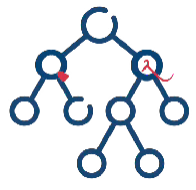
\includegraphics[height=0.9cm]{msca_logo.png}}%
  \end{center}
  \vspace{0.45cm}
  \begin{center}
    \begin{minipage}{0.1\textwidth}\centering
      \href{https://quantlet.com}{
\includegraphics[height=0.9cm]{ql_logo.png}}\end{minipage}%
    \begin{minipage}{0.78\textwidth}\centering
      {\Large\bfseries\usebeamercolor[fg]{title}\inserttitle}\par\vspace{0.25cm}
      {\large\usebeamercolor[fg]{title}\insertsubtitle}\end{minipage}%
    \begin{minipage}{0.1\textwidth}\centering
      \href{https://quantinar.com}{
\includegraphics[height=0.9cm]{qr_logo.png}}\end{minipage}
  \end{center}
  \vfill
  \hspace{0.4cm}{\bfseries\insertauthor}\par\vspace{0.12cm}
  \hspace{0.4cm}\begin{minipage}[t]{0.92\textwidth}\raggedright\footnotesize\insertinstitute\end{minipage}
  \par\vspace{0.4cm}}

% ---------------------------------------------------------------- lecture metadata
\newcommand{\nnshort}{}
\newcommand{\nnnb}{notebooks}
\newcommand{\nnrepo}{https://github.com/danpele/NEURAL_BIZ/tree/main}
% language-dependent labels (English default; \nnromanian switches to Romanian, call it before \nnlecture)
\newcommand{\txtcourse}{Neural Networks and Deep Learning}
\newcommand{\txtlecture}{Lecture}
\newcommand{\txtoutline}{Outline}
\newcommand{\txtintuition}{In one sentence:}
\newcommand{\txtjob}{In practice:}
\newcommand{\txttry}{Experiment yourself:}
\newcommand{\txtwhere}{where}
\newcommand{\txtsim}{SIMULATED DATA (teaching illustration)}
\newcommand{\txtnbsuffix}{}
\newcommand{\txtinstitute}{Bucharest University of Economic Studies (ASE), Department of Statistics and Econometrics\\
    Romanian Academy, Institute for Economic Forecasting (IPE)\\
    IDA Institute Digital Assets \textbullet\ AI4EFin \textbullet\ MSCA Digital Finance}
\newcommand{\nnromanian}{%
  \renewcommand{\txtcourse}{Rețele neuronale și deep learning}%
  \renewcommand{\txtlecture}{Cursul}%
  \renewcommand{\txtoutline}{Cuprins}%
  \renewcommand{\txtintuition}{Pe scurt:}%
  \renewcommand{\txtjob}{În practică:}%
  \renewcommand{\txttry}{Exercițiu practic:}%
  \renewcommand{\txtwhere}{unde}%
  \renewcommand{\txtsim}{DATE SIMULATE (doar pentru ilustrare)}%
  \renewcommand{\txtnbsuffix}{\string_ro}%
  \renewcommand{\txtinstitute}{Academia de Studii Economice din București (ASE), Departamentul de Statistică și Econometrie\\
    Academia Română, Institutul de Prognoză Economică (IPE)\\
    IDA Institute Digital Assets \textbullet\ AI4EFin \textbullet\ MSCA Digital Finance}}
\newcommand{\nnlecture}[2]{%
  \renewcommand{\nnshort}{\txtlecture\ #1}%
  \renewcommand{\nnnb}{notebooks/L#1\string_notebook\txtnbsuffix.ipynb}%
  \title[NN]{\txtcourse}%
  \subtitle{\txtlecture\ #1: #2}%
  \author{Prof.\ dr.\ Daniel Traian PELE}%
  \institute{\txtinstitute}%
  \date{}}

% ---------------------------------------------------------------- teaching blocks (one message per frame)
% \intuition{one plain sentence}  ->  formula with every symbol defined  ->  real-data example  ->  \manager{one line}
\newcommand{\intuition}[1]{\begin{itemize}\item {\color{MainBlue}\textbf{\txtintuition}}~#1\end{itemize}\vspace{0.6mm}}
\newcommand{\manager}[1]{\colorbox{Forest!10}{\parbox{\dimexpr\linewidth-2\fboxsep\relax}{\footnotesize
  \begin{itemize}\setlength{\itemsep}{0pt}\item \textbf{\color{Forest}\txtjob}~#1\end{itemize}}}}
% Experiment yourself: pointer to the matching notebook section
\newcommand{\tryit}[1]{{\scriptsize\href{\nnrepo/\nnnb}{%
  \raisebox{-0.15em}{
\includegraphics[height=0.85em]{ql_logo.png}}\,\textbf{\txttry}~\color{MainBlue}#1}}}
% bottom row: manager line (left) + experiment pointer (right), pinned to the bottom of the frame
\newcommand{\bottomrow}[2]{\par\vfill\noindent\begin{minipage}[b]{0.72\linewidth}#1\end{minipage}\hfill
  \begin{minipage}[b]{0.26\linewidth}\raggedleft #2\end{minipage}\par\vspace{0.5mm}}
\newcommand{\where}[1]{{\footnotesize\textbf{\txtwhere}~#1\par}}

% ---------------------------------------------------------------- helpers
% chart source line under a figure: \chartsource{Source ...; period ...}
\newcommand{\chartsource}[1]{\par\vspace{1pt}{\scriptsize\color{FooterGray}#1\par}}
% link to code: \quantlet{label}{path inside the repo}
\newcommand{\quantlet}[2]{\par\vspace{1pt}\hfill\href{\nnrepo/#2}{%
  \raisebox{-0.15em}{
\includegraphics[height=0.75em]{ql_logo.png}}\textcolor{MainBlue}{\scriptsize\ #1}}}
% inline Quantlet link for the bottom-right corner of a frame: \qlink{label}{path inside the repo}
\newcommand{\qlink}[2]{{\scriptsize\href{\nnrepo/#2}{\raisebox{-0.15em}{
\includegraphics[height=0.85em]{ql_logo.png}}\,\textcolor{MainBlue}{#1}}}}
\newcommand{\simlabel}{\colorbox{Crimson!12}{\scriptsize\bfseries\color{Crimson}\txtsim}}
\newcommand{\E}{\mathbb{E}}
\newcommand{\Var}{\operatorname{Var}}
\newcommand{\Cov}{\operatorname{Cov}}
\newcommand{\Corr}{\operatorname{Corr}}
\newcommand{\asinh}{\operatorname{asinh}}
\newcommand{\iid}{\overset{\text{i.i.d.}}{\sim}}
\newcommand{\EUR}{EUR}
% deep-learning notation (Bishop & Bishop, 2024): vectors bold lower case, matrices bold upper case
\newcommand{\R}{\mathbb{R}}
\newcommand{\vx}{\mathbf{x}}
\newcommand{\vy}{\mathbf{y}}
\newcommand{\vz}{\mathbf{z}}
\newcommand{\vh}{\mathbf{h}}
\newcommand{\vw}{\mathbf{w}}
\newcommand{\vb}{\mathbf{b}}
\newcommand{\mW}{\mathbf{W}}
\newcommand{\mX}{\mathbf{X}}
\newcommand{\btheta}{\boldsymbol{\theta}}
\newcommand{\loss}{\mathcal{L}}
\newcommand{\dataset}{\mathcal{D}}
\DeclareMathOperator*{\argmin}{arg\,min}
\DeclareMathOperator*{\argmax}{arg\,max}
\DeclareMathOperator{\softmax}{softmax}
\DeclareMathOperator{\ReLU}{ReLU}
\DeclareMathOperator{\sigm}{\sigma}

%   \nnlecture{k}{Lecture title}
% Logos live in lectures/common/logos/, charts in lectures/Lk/charts/.
% Do NOT add \hfuzz / \vfuzz / \hbadness here: overfull boxes must be fixed, not hidden.
% =============================================================================

\usetheme{default}
\setbeamersize{text margin left=7mm, text margin right=7mm}

% ---------------------------------------------------------------- packages
\usepackage[utf8]{inputenc}
\usepackage[T1]{fontenc}
\usepackage{lmodern}
\usepackage{amsmath, amssymb}
\usepackage{mathtools}
\usepackage{bm}
\usepackage{tikz}
\usetikzlibrary{arrows.meta, positioning, calc, shapes.misc}
\usepackage{booktabs}
\usepackage{array}
\usepackage{graphicx}
\usepackage{colortbl}
\usepackage{xcolor}
\usepackage{multicol}
\hypersetup{colorlinks=true, linkcolor=MainBlue, urlcolor=MainBlue, citecolor=MainBlue}
\graphicspath{{../common/logos/}}   % charts are included with their language folder: charts/en/, charts/ro/

% ---------------------------------------------------------------- colours
\definecolor{MainBlue}{RGB}{26, 58, 110}
\definecolor{IDAred}{RGB}{205, 0, 0}
\definecolor{DarkGray}{RGB}{51, 51, 51}
\definecolor{FooterGray}{RGB}{100, 100, 100}
\definecolor{BlockGray}{RGB}{236, 238, 242}
\definecolor{KeynoteGray}{RGB}{218, 218, 218}
\definecolor{Crimson}{RGB}{190, 40, 50}
\definecolor{Forest}{RGB}{30, 110, 50}
\definecolor{Bitter}{RGB}{214, 150, 20}
% chart palette (same hex values and order as lectures/common/nn_plot.py SERIES)
\definecolor{Ser1}{HTML}{2A78D6}
\definecolor{Ser2}{HTML}{EB6834}
\definecolor{Ser3}{HTML}{1BAF7A}
\definecolor{Ser4}{HTML}{EDA100}
\definecolor{Ser5}{HTML}{E87BA4}
\definecolor{Ser6}{HTML}{008300}
\definecolor{Ser7}{HTML}{6250D6}
\definecolor{Ser8}{HTML}{E34948}

\setbeamertemplate{background}{%
  \begin{tikzpicture}[remember picture, overlay]
    \shade[shading=axis, shading angle=315, top color=white, bottom color=KeynoteGray]
      (current page.south west) rectangle (current page.north east);
  \end{tikzpicture}}
\setbeamercolor{background canvas}{bg=}
\setbeamercolor{structure}{fg=MainBlue}
\setbeamercolor{normal text}{fg=DarkGray}
\setbeamercolor{title}{fg=IDAred}
\setbeamercolor{frametitle}{fg=IDAred, bg=}
\setbeamercolor{block title}{bg=MainBlue, fg=white}
\setbeamercolor{block body}{bg=BlockGray, fg=DarkGray}
\setbeamercolor{block title alerted}{bg=Crimson, fg=white}
\setbeamercolor{block body alerted}{bg=Crimson!7, fg=DarkGray}
\setbeamercolor{block title example}{bg=Forest, fg=white}
\setbeamercolor{block body example}{bg=Forest!7, fg=DarkGray}
\setbeamercolor{item}{fg=MainBlue}
\setbeamerfont{frametitle}{size=\large, series=\bfseries}
\setbeamerfont{block title}{size=\small, series=\bfseries}
\setbeamertemplate{blocks}[rounded][shadow=false]
\setbeamertemplate{itemize item}{\color{MainBlue}$\boxdot$}
\setbeamertemplate{itemize subitem}{\color{MainBlue}\scriptsize$\blacktriangleright$}
% compact two-level lists: level 1 = main point, level 2 = details (no text outside bullets)
\setbeamerfont{itemize/enumerate subbody}{size=\footnotesize}
\setlength{\leftmargini}{1.1em}
\setlength{\leftmarginii}{1.1em}
\setbeamertemplate{itemize/enumerate body begin}{\setlength{\topsep}{0pt}\setlength{\partopsep}{0pt}\setlength{\parskip}{0pt}}
\setbeamertemplate{itemize/enumerate subbody begin}{\setlength{\topsep}{0pt}\setlength{\partopsep}{0pt}\setlength{\itemsep}{0pt}\vspace{-0.4ex}}

\setbeamertemplate{enumerate item}{\color{MainBlue}\insertenumlabel.}
\setlength{\leftmargini}{1.3em}
\setlength{\leftmarginii}{1.2em}
\setbeamertemplate{navigation symbols}{}
\setbeamertemplate{section in toc}{\color{MainBlue}$\blacktriangleright$~\inserttocsection}
\setbeamertemplate{caption}{\raggedright\insertcaption\par}
% frame subtitle = precise citation line under the claim title (Weron style)
\setbeamerfont{framesubtitle}{size=\footnotesize}
\setbeamercolor{framesubtitle}{fg=FooterGray}
% outline that reappears at every section with the current section highlighted
\setbeamertemplate{section in toc shaded}[default][35]
\setbeamertemplate{subsection in toc shaded}[default][35]
\setbeamertemplate{subsection in toc}{\leavevmode\leftskip=2.2em\color{DarkGray}\small\inserttocsubsection\par}
\AtBeginSection[]{{\begin{frame}{\txtoutline}\vspace{2mm}\small
  \tableofcontents[currentsection,hideothersubsections]\end{frame}}}

% ---------------------------------------------------------------- head and foot
\setbeamertemplate{headline}{%
  \vskip10pt%
  \hbox to \paperwidth{\hskip0.5cm%
    {\small\color{FooterGray}\renewcommand{\hyperlink}[2]{##2}\insertsectionhead}%
    \hfill\textcolor{FooterGray}{\small\insertframenumber}\hskip0.5cm}%
  \vskip4pt{\color{FooterGray}\hrule height 0.4pt}}
% footer as in the other courses (MFM, SFM): course name on the left, small sparkline on the right
\setbeamertemplate{footline}{%
  {\color{FooterGray}\hrule height 0.4pt}\vskip4pt%
  \hbox to \paperwidth{\hskip0.5cm%
    \textcolor{FooterGray}{\small\txtcourse}%
    \hfill\raisebox{-0.1em}{\begin{tikzpicture}[x=0.08em, y=0.08em, line width=0.4pt]
      \draw[FooterGray] (0,3) -- (1,4) -- (2,3.5) -- (3,5) -- (4,4) -- (5,6) -- (6,5.5) -- (7,4) -- (8,5) -- (9,7) -- (10,6) -- (11,5) -- (12,6.5) -- (13,8) -- (14,7) -- (15,6) -- (16,7.5) -- (17,9) -- (18,8) -- (19,7) -- (20,8.5) -- (21,10) -- (22,9) -- (23,8) -- (24,9.5);
    \end{tikzpicture}}\hskip0.5cm}%
  \vskip6pt}

% ---------------------------------------------------------------- title page
\defbeamertemplate*{title page}{nn}[1][]{%
  \vspace{0.15cm}
  \begin{center}
    \href{https://www.ase.ro}{
\includegraphics[height=0.9cm]{ase_logo.png}}\hspace{0.3cm}%
    \href{https://ipe.ro/new}{
\includegraphics[height=0.9cm]{acad_logo.png}}\hspace{0.3cm}%
    \href{https://theida.net}{
\includegraphics[height=0.9cm]{ida_logo.png}}\hspace{0.3cm}%
    \href{https://blockchain-research-center.com}{
\includegraphics[height=0.9cm]{brc_logo.png}}\hspace{0.3cm}%
    \href{https://www.ai4efin.ase.ro}{
\includegraphics[height=0.9cm]{ai4efin_logo.png}}\hspace{0.3cm}%
    \href{https://www.digital-finance-msca.com}{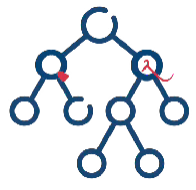
\includegraphics[height=0.9cm]{msca_logo.png}}%
  \end{center}
  \vspace{0.45cm}
  \begin{center}
    \begin{minipage}{0.1\textwidth}\centering
      \href{https://quantlet.com}{
\includegraphics[height=0.9cm]{ql_logo.png}}\end{minipage}%
    \begin{minipage}{0.78\textwidth}\centering
      {\Large\bfseries\usebeamercolor[fg]{title}\inserttitle}\par\vspace{0.25cm}
      {\large\usebeamercolor[fg]{title}\insertsubtitle}\end{minipage}%
    \begin{minipage}{0.1\textwidth}\centering
      \href{https://quantinar.com}{
\includegraphics[height=0.9cm]{qr_logo.png}}\end{minipage}
  \end{center}
  \vfill
  \hspace{0.4cm}{\bfseries\insertauthor}\par\vspace{0.12cm}
  \hspace{0.4cm}\begin{minipage}[t]{0.92\textwidth}\raggedright\footnotesize\insertinstitute\end{minipage}
  \par\vspace{0.4cm}}

% ---------------------------------------------------------------- lecture metadata
\newcommand{\nnshort}{}
\newcommand{\nnnb}{notebooks}
\newcommand{\nnrepo}{https://github.com/danpele/NEURAL_BIZ/tree/main}
% language-dependent labels (English default; \nnromanian switches to Romanian, call it before \nnlecture)
\newcommand{\txtcourse}{Neural Networks and Deep Learning}
\newcommand{\txtlecture}{Lecture}
\newcommand{\txtoutline}{Outline}
\newcommand{\txtintuition}{In one sentence:}
\newcommand{\txtjob}{In practice:}
\newcommand{\txttry}{Experiment yourself:}
\newcommand{\txtwhere}{where}
\newcommand{\txtsim}{SIMULATED DATA (teaching illustration)}
\newcommand{\txtnbsuffix}{}
\newcommand{\txtinstitute}{Bucharest University of Economic Studies (ASE), Department of Statistics and Econometrics\\
    Romanian Academy, Institute for Economic Forecasting (IPE)\\
    IDA Institute Digital Assets \textbullet\ AI4EFin \textbullet\ MSCA Digital Finance}
\newcommand{\nnromanian}{%
  \renewcommand{\txtcourse}{Rețele neuronale și deep learning}%
  \renewcommand{\txtlecture}{Cursul}%
  \renewcommand{\txtoutline}{Cuprins}%
  \renewcommand{\txtintuition}{Pe scurt:}%
  \renewcommand{\txtjob}{În practică:}%
  \renewcommand{\txttry}{Exercițiu practic:}%
  \renewcommand{\txtwhere}{unde}%
  \renewcommand{\txtsim}{DATE SIMULATE (doar pentru ilustrare)}%
  \renewcommand{\txtnbsuffix}{\string_ro}%
  \renewcommand{\txtinstitute}{Academia de Studii Economice din București (ASE), Departamentul de Statistică și Econometrie\\
    Academia Română, Institutul de Prognoză Economică (IPE)\\
    IDA Institute Digital Assets \textbullet\ AI4EFin \textbullet\ MSCA Digital Finance}}
\newcommand{\nnlecture}[2]{%
  \renewcommand{\nnshort}{\txtlecture\ #1}%
  \renewcommand{\nnnb}{notebooks/L#1\string_notebook\txtnbsuffix.ipynb}%
  \title[NN]{\txtcourse}%
  \subtitle{\txtlecture\ #1: #2}%
  \author{Prof.\ dr.\ Daniel Traian PELE}%
  \institute{\txtinstitute}%
  \date{}}

% ---------------------------------------------------------------- teaching blocks (one message per frame)
% \intuition{one plain sentence}  ->  formula with every symbol defined  ->  real-data example  ->  \manager{one line}
\newcommand{\intuition}[1]{\begin{itemize}\item {\color{MainBlue}\textbf{\txtintuition}}~#1\end{itemize}\vspace{0.6mm}}
\newcommand{\manager}[1]{\colorbox{Forest!10}{\parbox{\dimexpr\linewidth-2\fboxsep\relax}{\footnotesize
  \begin{itemize}\setlength{\itemsep}{0pt}\item \textbf{\color{Forest}\txtjob}~#1\end{itemize}}}}
% Experiment yourself: pointer to the matching notebook section
\newcommand{\tryit}[1]{{\scriptsize\href{\nnrepo/\nnnb}{%
  \raisebox{-0.15em}{
\includegraphics[height=0.85em]{ql_logo.png}}\,\textbf{\txttry}~\color{MainBlue}#1}}}
% bottom row: manager line (left) + experiment pointer (right), pinned to the bottom of the frame
\newcommand{\bottomrow}[2]{\par\vfill\noindent\begin{minipage}[b]{0.72\linewidth}#1\end{minipage}\hfill
  \begin{minipage}[b]{0.26\linewidth}\raggedleft #2\end{minipage}\par\vspace{0.5mm}}
\newcommand{\where}[1]{{\footnotesize\textbf{\txtwhere}~#1\par}}

% ---------------------------------------------------------------- helpers
% chart source line under a figure: \chartsource{Source ...; period ...}
\newcommand{\chartsource}[1]{\par\vspace{1pt}{\scriptsize\color{FooterGray}#1\par}}
% link to code: \quantlet{label}{path inside the repo}
\newcommand{\quantlet}[2]{\par\vspace{1pt}\hfill\href{\nnrepo/#2}{%
  \raisebox{-0.15em}{
\includegraphics[height=0.75em]{ql_logo.png}}\textcolor{MainBlue}{\scriptsize\ #1}}}
% inline Quantlet link for the bottom-right corner of a frame: \qlink{label}{path inside the repo}
\newcommand{\qlink}[2]{{\scriptsize\href{\nnrepo/#2}{\raisebox{-0.15em}{
\includegraphics[height=0.85em]{ql_logo.png}}\,\textcolor{MainBlue}{#1}}}}
\newcommand{\simlabel}{\colorbox{Crimson!12}{\scriptsize\bfseries\color{Crimson}\txtsim}}
\newcommand{\E}{\mathbb{E}}
\newcommand{\Var}{\operatorname{Var}}
\newcommand{\Cov}{\operatorname{Cov}}
\newcommand{\Corr}{\operatorname{Corr}}
\newcommand{\asinh}{\operatorname{asinh}}
\newcommand{\iid}{\overset{\text{i.i.d.}}{\sim}}
\newcommand{\EUR}{EUR}
% deep-learning notation (Bishop & Bishop, 2024): vectors bold lower case, matrices bold upper case
\newcommand{\R}{\mathbb{R}}
\newcommand{\vx}{\mathbf{x}}
\newcommand{\vy}{\mathbf{y}}
\newcommand{\vz}{\mathbf{z}}
\newcommand{\vh}{\mathbf{h}}
\newcommand{\vw}{\mathbf{w}}
\newcommand{\vb}{\mathbf{b}}
\newcommand{\mW}{\mathbf{W}}
\newcommand{\mX}{\mathbf{X}}
\newcommand{\btheta}{\boldsymbol{\theta}}
\newcommand{\loss}{\mathcal{L}}
\newcommand{\dataset}{\mathcal{D}}
\DeclareMathOperator*{\argmin}{arg\,min}
\DeclareMathOperator*{\argmax}{arg\,max}
\DeclareMathOperator{\softmax}{softmax}
\DeclareMathOperator{\ReLU}{ReLU}
\DeclareMathOperator{\sigm}{\sigma}

%   \nnlecture{k}{Lecture title}
% Logos live in lectures/common/logos/, charts in lectures/Lk/charts/.
% Do NOT add \hfuzz / \vfuzz / \hbadness here: overfull boxes must be fixed, not hidden.
% =============================================================================

\usetheme{default}
\setbeamersize{text margin left=7mm, text margin right=7mm}

% ---------------------------------------------------------------- packages
\usepackage[utf8]{inputenc}
\usepackage[T1]{fontenc}
\usepackage{lmodern}
\usepackage{amsmath, amssymb}
\usepackage{mathtools}
\usepackage{bm}
\usepackage{tikz}
\usetikzlibrary{arrows.meta, positioning, calc, shapes.misc}
\usepackage{booktabs}
\usepackage{array}
\usepackage{graphicx}
\usepackage{colortbl}
\usepackage{xcolor}
\usepackage{multicol}
\hypersetup{colorlinks=true, linkcolor=MainBlue, urlcolor=MainBlue, citecolor=MainBlue}
\graphicspath{{../common/logos/}}   % charts are included with their language folder: charts/en/, charts/ro/

% ---------------------------------------------------------------- colours
\definecolor{MainBlue}{RGB}{26, 58, 110}
\definecolor{IDAred}{RGB}{205, 0, 0}
\definecolor{DarkGray}{RGB}{51, 51, 51}
\definecolor{FooterGray}{RGB}{100, 100, 100}
\definecolor{BlockGray}{RGB}{236, 238, 242}
\definecolor{KeynoteGray}{RGB}{218, 218, 218}
\definecolor{Crimson}{RGB}{190, 40, 50}
\definecolor{Forest}{RGB}{30, 110, 50}
\definecolor{Bitter}{RGB}{214, 150, 20}
% chart palette (same hex values and order as lectures/common/nn_plot.py SERIES)
\definecolor{Ser1}{HTML}{2A78D6}
\definecolor{Ser2}{HTML}{EB6834}
\definecolor{Ser3}{HTML}{1BAF7A}
\definecolor{Ser4}{HTML}{EDA100}
\definecolor{Ser5}{HTML}{E87BA4}
\definecolor{Ser6}{HTML}{008300}
\definecolor{Ser7}{HTML}{6250D6}
\definecolor{Ser8}{HTML}{E34948}

\setbeamertemplate{background}{%
  \begin{tikzpicture}[remember picture, overlay]
    \shade[shading=axis, shading angle=315, top color=white, bottom color=KeynoteGray]
      (current page.south west) rectangle (current page.north east);
  \end{tikzpicture}}
\setbeamercolor{background canvas}{bg=}
\setbeamercolor{structure}{fg=MainBlue}
\setbeamercolor{normal text}{fg=DarkGray}
\setbeamercolor{title}{fg=IDAred}
\setbeamercolor{frametitle}{fg=IDAred, bg=}
\setbeamercolor{block title}{bg=MainBlue, fg=white}
\setbeamercolor{block body}{bg=BlockGray, fg=DarkGray}
\setbeamercolor{block title alerted}{bg=Crimson, fg=white}
\setbeamercolor{block body alerted}{bg=Crimson!7, fg=DarkGray}
\setbeamercolor{block title example}{bg=Forest, fg=white}
\setbeamercolor{block body example}{bg=Forest!7, fg=DarkGray}
\setbeamercolor{item}{fg=MainBlue}
\setbeamerfont{frametitle}{size=\large, series=\bfseries}
\setbeamerfont{block title}{size=\small, series=\bfseries}
\setbeamertemplate{blocks}[rounded][shadow=false]
\setbeamertemplate{itemize item}{\color{MainBlue}$\boxdot$}
\setbeamertemplate{itemize subitem}{\color{MainBlue}\scriptsize$\blacktriangleright$}
% compact two-level lists: level 1 = main point, level 2 = details (no text outside bullets)
\setbeamerfont{itemize/enumerate subbody}{size=\footnotesize}
\setlength{\leftmargini}{1.1em}
\setlength{\leftmarginii}{1.1em}
\setbeamertemplate{itemize/enumerate body begin}{\setlength{\topsep}{0pt}\setlength{\partopsep}{0pt}\setlength{\parskip}{0pt}}
\setbeamertemplate{itemize/enumerate subbody begin}{\setlength{\topsep}{0pt}\setlength{\partopsep}{0pt}\setlength{\itemsep}{0pt}\vspace{-0.4ex}}

\setbeamertemplate{enumerate item}{\color{MainBlue}\insertenumlabel.}
\setlength{\leftmargini}{1.3em}
\setlength{\leftmarginii}{1.2em}
\setbeamertemplate{navigation symbols}{}
\setbeamertemplate{section in toc}{\color{MainBlue}$\blacktriangleright$~\inserttocsection}
\setbeamertemplate{caption}{\raggedright\insertcaption\par}
% frame subtitle = precise citation line under the claim title (Weron style)
\setbeamerfont{framesubtitle}{size=\footnotesize}
\setbeamercolor{framesubtitle}{fg=FooterGray}
% outline that reappears at every section with the current section highlighted
\setbeamertemplate{section in toc shaded}[default][35]
\setbeamertemplate{subsection in toc shaded}[default][35]
\setbeamertemplate{subsection in toc}{\leavevmode\leftskip=2.2em\color{DarkGray}\small\inserttocsubsection\par}
\AtBeginSection[]{{\begin{frame}{\txtoutline}\vspace{2mm}\small
  \tableofcontents[currentsection,hideothersubsections]\end{frame}}}

% ---------------------------------------------------------------- head and foot
\setbeamertemplate{headline}{%
  \vskip10pt%
  \hbox to \paperwidth{\hskip0.5cm%
    {\small\color{FooterGray}\renewcommand{\hyperlink}[2]{##2}\insertsectionhead}%
    \hfill\textcolor{FooterGray}{\small\insertframenumber}\hskip0.5cm}%
  \vskip4pt{\color{FooterGray}\hrule height 0.4pt}}
% footer as in the other courses (MFM, SFM): course name on the left, small sparkline on the right
\setbeamertemplate{footline}{%
  {\color{FooterGray}\hrule height 0.4pt}\vskip4pt%
  \hbox to \paperwidth{\hskip0.5cm%
    \textcolor{FooterGray}{\small\txtcourse}%
    \hfill\raisebox{-0.1em}{\begin{tikzpicture}[x=0.08em, y=0.08em, line width=0.4pt]
      \draw[FooterGray] (0,3) -- (1,4) -- (2,3.5) -- (3,5) -- (4,4) -- (5,6) -- (6,5.5) -- (7,4) -- (8,5) -- (9,7) -- (10,6) -- (11,5) -- (12,6.5) -- (13,8) -- (14,7) -- (15,6) -- (16,7.5) -- (17,9) -- (18,8) -- (19,7) -- (20,8.5) -- (21,10) -- (22,9) -- (23,8) -- (24,9.5);
    \end{tikzpicture}}\hskip0.5cm}%
  \vskip6pt}

% ---------------------------------------------------------------- title page
\defbeamertemplate*{title page}{nn}[1][]{%
  \vspace{0.15cm}
  \begin{center}
    \href{https://www.ase.ro}{
\includegraphics[height=0.9cm]{ase_logo.png}}\hspace{0.3cm}%
    \href{https://ipe.ro/new}{
\includegraphics[height=0.9cm]{acad_logo.png}}\hspace{0.3cm}%
    \href{https://theida.net}{
\includegraphics[height=0.9cm]{ida_logo.png}}\hspace{0.3cm}%
    \href{https://blockchain-research-center.com}{
\includegraphics[height=0.9cm]{brc_logo.png}}\hspace{0.3cm}%
    \href{https://www.ai4efin.ase.ro}{
\includegraphics[height=0.9cm]{ai4efin_logo.png}}\hspace{0.3cm}%
    \href{https://www.digital-finance-msca.com}{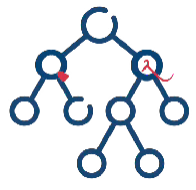
\includegraphics[height=0.9cm]{msca_logo.png}}%
  \end{center}
  \vspace{0.45cm}
  \begin{center}
    \begin{minipage}{0.1\textwidth}\centering
      \href{https://quantlet.com}{
\includegraphics[height=0.9cm]{ql_logo.png}}\end{minipage}%
    \begin{minipage}{0.78\textwidth}\centering
      {\Large\bfseries\usebeamercolor[fg]{title}\inserttitle}\par\vspace{0.25cm}
      {\large\usebeamercolor[fg]{title}\insertsubtitle}\end{minipage}%
    \begin{minipage}{0.1\textwidth}\centering
      \href{https://quantinar.com}{
\includegraphics[height=0.9cm]{qr_logo.png}}\end{minipage}
  \end{center}
  \vfill
  \hspace{0.4cm}{\bfseries\insertauthor}\par\vspace{0.12cm}
  \hspace{0.4cm}\begin{minipage}[t]{0.92\textwidth}\raggedright\footnotesize\insertinstitute\end{minipage}
  \par\vspace{0.4cm}}

% ---------------------------------------------------------------- lecture metadata
\newcommand{\nnshort}{}
\newcommand{\nnnb}{notebooks}
\newcommand{\nnrepo}{https://github.com/danpele/NEURAL_BIZ/tree/main}
% language-dependent labels (English default; \nnromanian switches to Romanian, call it before \nnlecture)
\newcommand{\txtcourse}{Neural Networks and Deep Learning}
\newcommand{\txtlecture}{Lecture}
\newcommand{\txtoutline}{Outline}
\newcommand{\txtintuition}{In one sentence:}
\newcommand{\txtjob}{In practice:}
\newcommand{\txttry}{Experiment yourself:}
\newcommand{\txtwhere}{where}
\newcommand{\txtsim}{SIMULATED DATA (teaching illustration)}
\newcommand{\txtnbsuffix}{}
\newcommand{\txtinstitute}{Bucharest University of Economic Studies (ASE), Department of Statistics and Econometrics\\
    Romanian Academy, Institute for Economic Forecasting (IPE)\\
    IDA Institute Digital Assets \textbullet\ AI4EFin \textbullet\ MSCA Digital Finance}
\newcommand{\nnromanian}{%
  \renewcommand{\txtcourse}{Rețele neuronale și deep learning}%
  \renewcommand{\txtlecture}{Cursul}%
  \renewcommand{\txtoutline}{Cuprins}%
  \renewcommand{\txtintuition}{Pe scurt:}%
  \renewcommand{\txtjob}{În practică:}%
  \renewcommand{\txttry}{Exercițiu practic:}%
  \renewcommand{\txtwhere}{unde}%
  \renewcommand{\txtsim}{DATE SIMULATE (doar pentru ilustrare)}%
  \renewcommand{\txtnbsuffix}{\string_ro}%
  \renewcommand{\txtinstitute}{Academia de Studii Economice din București (ASE), Departamentul de Statistică și Econometrie\\
    Academia Română, Institutul de Prognoză Economică (IPE)\\
    IDA Institute Digital Assets \textbullet\ AI4EFin \textbullet\ MSCA Digital Finance}}
\newcommand{\nnlecture}[2]{%
  \renewcommand{\nnshort}{\txtlecture\ #1}%
  \renewcommand{\nnnb}{notebooks/L#1\string_notebook\txtnbsuffix.ipynb}%
  \title[NN]{\txtcourse}%
  \subtitle{\txtlecture\ #1: #2}%
  \author{Prof.\ dr.\ Daniel Traian PELE}%
  \institute{\txtinstitute}%
  \date{}}

% ---------------------------------------------------------------- teaching blocks (one message per frame)
% \intuition{one plain sentence}  ->  formula with every symbol defined  ->  real-data example  ->  \manager{one line}
\newcommand{\intuition}[1]{\begin{itemize}\item {\color{MainBlue}\textbf{\txtintuition}}~#1\end{itemize}\vspace{0.6mm}}
\newcommand{\manager}[1]{\colorbox{Forest!10}{\parbox{\dimexpr\linewidth-2\fboxsep\relax}{\footnotesize
  \begin{itemize}\setlength{\itemsep}{0pt}\item \textbf{\color{Forest}\txtjob}~#1\end{itemize}}}}
% Experiment yourself: pointer to the matching notebook section
\newcommand{\tryit}[1]{{\scriptsize\href{\nnrepo/\nnnb}{%
  \raisebox{-0.15em}{
\includegraphics[height=0.85em]{ql_logo.png}}\,\textbf{\txttry}~\color{MainBlue}#1}}}
% bottom row: manager line (left) + experiment pointer (right), pinned to the bottom of the frame
\newcommand{\bottomrow}[2]{\par\vfill\noindent\begin{minipage}[b]{0.72\linewidth}#1\end{minipage}\hfill
  \begin{minipage}[b]{0.26\linewidth}\raggedleft #2\end{minipage}\par\vspace{0.5mm}}
\newcommand{\where}[1]{{\footnotesize\textbf{\txtwhere}~#1\par}}

% ---------------------------------------------------------------- helpers
% chart source line under a figure: \chartsource{Source ...; period ...}
\newcommand{\chartsource}[1]{\par\vspace{1pt}{\scriptsize\color{FooterGray}#1\par}}
% link to code: \quantlet{label}{path inside the repo}
\newcommand{\quantlet}[2]{\par\vspace{1pt}\hfill\href{\nnrepo/#2}{%
  \raisebox{-0.15em}{
\includegraphics[height=0.75em]{ql_logo.png}}\textcolor{MainBlue}{\scriptsize\ #1}}}
% inline Quantlet link for the bottom-right corner of a frame: \qlink{label}{path inside the repo}
\newcommand{\qlink}[2]{{\scriptsize\href{\nnrepo/#2}{\raisebox{-0.15em}{
\includegraphics[height=0.85em]{ql_logo.png}}\,\textcolor{MainBlue}{#1}}}}
\newcommand{\simlabel}{\colorbox{Crimson!12}{\scriptsize\bfseries\color{Crimson}\txtsim}}
\newcommand{\E}{\mathbb{E}}
\newcommand{\Var}{\operatorname{Var}}
\newcommand{\Cov}{\operatorname{Cov}}
\newcommand{\Corr}{\operatorname{Corr}}
\newcommand{\asinh}{\operatorname{asinh}}
\newcommand{\iid}{\overset{\text{i.i.d.}}{\sim}}
\newcommand{\EUR}{EUR}
% deep-learning notation (Bishop & Bishop, 2024): vectors bold lower case, matrices bold upper case
\newcommand{\R}{\mathbb{R}}
\newcommand{\vx}{\mathbf{x}}
\newcommand{\vy}{\mathbf{y}}
\newcommand{\vz}{\mathbf{z}}
\newcommand{\vh}{\mathbf{h}}
\newcommand{\vw}{\mathbf{w}}
\newcommand{\vb}{\mathbf{b}}
\newcommand{\mW}{\mathbf{W}}
\newcommand{\mX}{\mathbf{X}}
\newcommand{\btheta}{\boldsymbol{\theta}}
\newcommand{\loss}{\mathcal{L}}
\newcommand{\dataset}{\mathcal{D}}
\DeclareMathOperator*{\argmin}{arg\,min}
\DeclareMathOperator*{\argmax}{arg\,max}
\DeclareMathOperator{\softmax}{softmax}
\DeclareMathOperator{\ReLU}{ReLU}
\DeclareMathOperator{\sigm}{\sigma}

\usepackage[romanian]{babel}
\nnromanian
\nnlecture{6}{Bazele NLP: reprezentarea textului și reprezentarea vectorială a cuvintelor}
\begin{document}
{\setbeamertemplate{headline}{}\setbeamertemplate{footline}{}
\begin{frame}\titlepage\end{frame}}
% END-FRONT-MATTER

\begin{frame}{Obiectivele cursului}
\small
\begin{itemize}\setlength{\itemsep}{4pt}
  \item Să transformați textul financiar în numere pentru prelucrarea limbajului natural (NLP): unități lexicale, vocabular, sac de cuvinte și frecvența termenului--frecvența inversă în documente (TF-IDF).
  \item Să scrieți funcțiile-obiectiv ale word2vec și GloVe și să le antrenați pe un corpus real de discursuri ale băncii centrale.
  \item Să construiți clasificatoare de fraze din reprezentări rare și dense, cu modele de referință și teste corecte.
  \item Să măsurați sentimentul și temele financiare în știri și tweet-uri și să știți cînd un model liniar este suficient.
\end{itemize}
\end{frame}

% BEGIN-ABBR

\begin{frame}{Abrevieri}
\small
\vspace{-1mm}\begin{columns}[T,onlytextwidth]
\begin{column}{0.49\textwidth}{\scriptsize\renewcommand{\arraystretch}{0.96}\begin{tabular}{@{}>{\bfseries}l@{\ \ }p{0.74\linewidth}@{}}AI & inteligență artificială\\
ASE & Academia de Studii Economice din București\\
BCE & Banca Centrală Europeană\\
BERT & reprezentări bidirecționale ale codificatorului transformer (BERT)\\
BoW & sac de cuvinte (bag of words)\\
CBOW & sac continuu de cuvinte (varianta word2vec)\\
CPU & procesor central\\
ES & pierderea medie așteptată peste VaR (expected shortfall)\\
ESG & mediu, social și guvernanță\\
FinBERT & model BERT adaptat textelor financiare\\
IPE & Institutul de Prognoză Economică, Academia Română\\\end{tabular}}\end{column}
\begin{column}{0.49\textwidth}{\scriptsize\renewcommand{\arraystretch}{0.96}\begin{tabular}{@{}>{\bfseries}l@{\ \ }p{0.74\linewidth}@{}}LLM & model lingvistic mare\\
MLP & perceptron multistrat\\
NLP & prelucrarea limbajului natural\\
OOV & în afara vocabularului\\
PCA & analiza componentelor principale\\
PMI & informația mutuală punctuală\\
SGNS & skip-gram cu eșantionare negativă\\
SVD & descompunerea în valori singulare\\
TF-IDF & frecvența termenului--frecvența inversă în documente\\
VaR & valoarea expusă la risc (value-at-risk)\\\end{tabular}}\end{column}
\end{columns}
\end{frame}

% END-ABBR

\begin{frame}{Numai date reale: trei colecții de texte}
\footnotesize
{\footnotesize\renewcommand{\arraystretch}{1.05}\setlength{\tabcolsep}{4pt}
\begin{tabular}{@{}p{0.23\textwidth}p{0.33\textwidth}p{0.17\textwidth}p{0.18\textwidth}@{}}\toprule
Corpusul & Conținut & Dimensiune & Utilizare aici \\ \midrule
Financial PhraseBank & fraze din știri financiare despre companii listate în Finlanda, etichetate pozitiv / neutru / negativ de 5--8 adnotatori & 4\,838 de fraze & sentiment \\
Twitter financial news & tweet-uri financiare: pesimist / optimist / neutru și 20 de teme & 9\,543 + 2\,388 (sentiment), 16\,990 + 4\,117 (teme) & sentiment, teme \\
Discursurile Băncii Centrale Europene (BCE) & textele integrale ale membrilor Comitetului executiv și ai Consiliului de supraveghere & 400 de discursuri, 1\,289\,896 de unități lexicale & propriii noștri vectori de cuvinte \\
\bottomrule\end{tabular}}
\par\vspace{0.5mm}{\scriptsize \begin{itemize}\setlength{\itemsep}{0pt}
  \item Discursuri din perioada 8 ianuarie 2022 -- 30 octombrie 2026; PhraseBank de Malo et al. (2014); tweet-urile așa cum sînt publicate pe Hugging Face (seturile de antrenare și de validare).
  \item Fiecare model este antrenat pe procesorul central (CPU) al unui laptop, cu sămînța 20261108; seturile de test sînt folosite o singură dată.
\end{itemize}}
\par\vfill\noindent{\scriptsize\color{FooterGray}(data/SOURCES.md)}\par\vspace{0.5mm}
\end{frame}


\section{Textul ca date}

\begin{frame}{De la o frază la unități lexicale}
\footnotesize
\begin{itemize}\setlength{\itemsep}{4pt}
  \item \textbf{O frază reală din PhraseBank}
    \begin{itemize}\setlength{\itemsep}{0pt}
      \item ``Finnish Aktia Group 's operating profit rose to EUR 17.5 mn in the first quarter of 2010 from EUR 8.2 mn in the first quarter of 2009 .''
      \item Eticheta dată de adnotatori: \textbf{pozitiv}
    \end{itemize}
  \item \textbf{Tokenizatorul nostru}
    \begin{itemize}\setlength{\itemsep}{0pt}
      \item Litere mici, cuvinte și numere; fiecare număr devine \texttt{\textless{}num\textgreater{}}; legăturile și mențiunile cu @ sînt eliminate
      \item Primele unități: \texttt{finnish aktia group s operating profit rose to eur \textless{}num\textgreater{} mn in the first} (27 în total)
    \end{itemize}
  \item \textbf{Alegeri care schimbă rezultatele}
    \begin{itemize}\setlength{\itemsep}{0pt}
      \item Trecerea la litere mici unește ``Bank'' și ``bank''; reducerea la rădăcină unește ``rose'' și ``rising''
      \item Eliminarea cuvintelor de legătură șterge ``not'', ``down'', ``up'': dăunător pentru sentiment
    \end{itemize}
\end{itemize}
\par\vfill\manager{documentați preprocesarea și păstrați-o identică în antrenare și în producție
    \begin{itemize}\setlength{\itemsep}{0pt}
      \item Un alt tokenizator înseamnă un alt model.
    \end{itemize}}\par\vspace{0.5mm}
\par\vfill\noindent{\scriptsize\color{FooterGray}(Malo et al., 2014)}\hfill\tryit{\S1}\par\vspace{0.5mm}
\end{frame}

\begin{frame}{Puține cuvinte sînt frecvente, cele mai multe sînt rare: legea lui Zipf}
\small
\intuition{în 400 de discursuri ale Băncii Centrale Europene, frecvența scade ca o putere a rangului.}
\vspace{-1mm}\[ f(r)\approx C\,r^{-a}\quad\Longleftrightarrow\quad\ln f(r)=\ln C-a\ln r \]\vspace{-2mm}
\begin{center}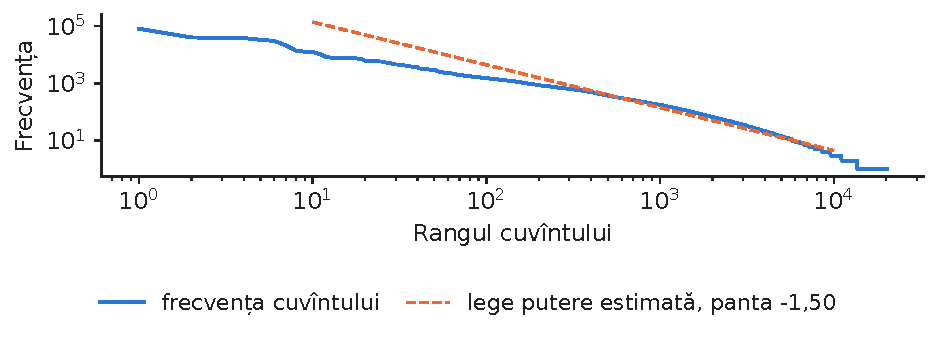
\includegraphics[width=\textwidth,height=0.360\textheight,keepaspectratio]{charts/ro/zipf.pdf}\end{center}\vspace{-3mm}
\chartsource{Sursa: Banca Centrală Europeană, setul de discursuri. Date: 8 ianuarie 2022 - 30 octombrie 2026, 400 de discursuri.}
\vspace{0.5mm}
\begin{itemize}\setlength{\itemsep}{0pt}
  \item 1\,289\,896 de unități lexicale, 20\,130 de cuvinte distincte
    \begin{itemize}\setlength{\itemsep}{0pt}
      \item Panta estimată \ensuremath{-}1{,}498 (rangurile 10 -- 10.000)
      \item Cele mai frecvente 10 cuvinte reprezintă 25{,}0\,\% din total.
    \end{itemize}
  \item 32{,}5\,\% dintre cuvintele distincte apar o singură dată: niciun model nu le poate învăța numai din acest corpus.
\end{itemize}
\par\vfill\noindent{\scriptsize\color{FooterGray}(Zipf, 1949; calcul propriu)}\hfill\qlink{NN\_L6\_zipf}{Quantlets/L6/NN_L6_zipf}\par\vspace{0.5mm}
\end{frame}


\section{Reprezentări rare: sacul de cuvinte și TF-IDF}

\begin{frame}{Sacul de cuvinte: un document este un vector de frecvențe}
\footnotesize
\intuition{ignorăm ordinea și păstrăm de cîte ori apare fiecare cuvînt din vocabular.}
\begin{columns}[T,onlytextwidth]
\begin{column}{0.53\textwidth}
\[ \mathbf x_i=(c_{i1},\dots,c_{iV})^{\top} \]\vspace{-2mm}\[ c_{ij}=\#\{\text{apariții ale cuvîntului } j \text{ în documentul } i\} \]{\footnotesize\begin{itemize}\setlength{\itemsep}{0pt}
  \item \textbf{\txtwhere}
    \begin{itemize}\setlength{\itemsep}{0pt}
      \item $V$ dimensiunea vocabularului (cuvintele întîlnite de cel puțin două ori în partea de antrenare)
      \item Matricea documente--termeni $\mathbf C\in\mathbb N^{n\times V}$ este aproape în întregime zero
    \end{itemize}
\end{itemize}\par}
\end{column}
\begin{column}{0.44\textwidth}
\begin{itemize}\setlength{\itemsep}{2pt}
  \item Sacul de cuvinte (BoW) + regresia logistică multinomială este modelul de referință standard pentru text.
  \item $n$-gramele adaugă ordinea locală: ``profit rose'' și ``profit fell'' devin trăsături.
  \item Vocabularul este construit numai din frazele de antrenare.
\end{itemize}
\end{column}
\end{columns}
\par\vfill\manager{modelele BoW sînt rapide, ieftine și explicabile cuvînt cu cuvînt: auditorilor le plac.}\par\vspace{0.5mm}
\par\vfill\noindent{\scriptsize\color{FooterGray}(Salton \& Buckley, 1988)}\par\vspace{0.5mm}
\end{frame}

\begin{frame}{TF-IDF: reducem ponderea cuvintelor care apar peste tot}
\footnotesize
\intuition{un cuvînt este informativ dacă este frecvent în acest document și rar în celelalte.}
\begin{columns}[T,onlytextwidth]
\begin{column}{0.53\textwidth}
\[ w_{ij}=\underbrace{(1+\ln c_{ij})}_{\text{tf}}\cdot\underbrace{\Big(\ln\frac{1+n}{1+n_j}+1\Big)}_{\text{idf}},\qquad \tilde{\mathbf x}_i=\frac{\mathbf w_i}{\|\mathbf w_i\|_2} \]{\footnotesize\begin{itemize}\setlength{\itemsep}{0pt}
  \item \textbf{\txtwhere}
    \begin{itemize}\setlength{\itemsep}{0pt}
      \item $c_{ij}>0$ frecvența termenului $j$ în documentul $i$ ($w_{ij}=0$ dacă $c_{ij}=0$)
      \item $n$ documente
      \item $n_j$ documente care conțin $j$
      \item Tf sublinear și idf netezit, ca în scikit-learn
    \end{itemize}
\end{itemize}\par}
\end{column}
\begin{column}{0.44\textwidth}
\begin{itemize}\setlength{\itemsep}{2pt}
  \item Frecvența termenului--frecvența inversă în documente (TF-IDF) pe unigrame și bigrame, apoi regresie logistică cu ponderi echilibrate ale claselor.
  \item Cuvinte ca ``the'', ``company'', \texttt{\textless{}num\textgreater{}} primesc un idf mic
    \begin{itemize}\setlength{\itemsep}{0pt}
      \item ``plunged'' unul mare.
    \end{itemize}
  \item Normalizarea $\ell_2$ face comparabile frazele lungi și cele scurte.
\end{itemize}
\end{column}
\end{columns}
\par\vfill\manager{TF-IDF + regresie logistică este modelul pe care orice furnizor de NLP trebuie să-l depășească pe documentele dumneavoastră.}\par\vspace{0.5mm}
\par\vfill\noindent{\scriptsize\color{FooterGray}(Salton \& Buckley, 1988)}\par\vspace{0.5mm}
\end{frame}

\begin{frame}{Modelul liniar învață un dicționar al sentimentului financiar}
\small
\intuition{diferența dintre coeficienții pozitiv și negativ ai fiecărui cuvînt, regresie logistică pe BoW, PhraseBank.}
\vspace{-1mm}\[ P(y=k\mid\mathbf x)=\frac{\exp(\boldsymbol\beta_k^{\top}\mathbf x+\alpha_k)}{\sum_{l}\exp(\boldsymbol\beta_l^{\top}\mathbf x+\alpha_l)} \]\vspace{-2mm}
\begin{center}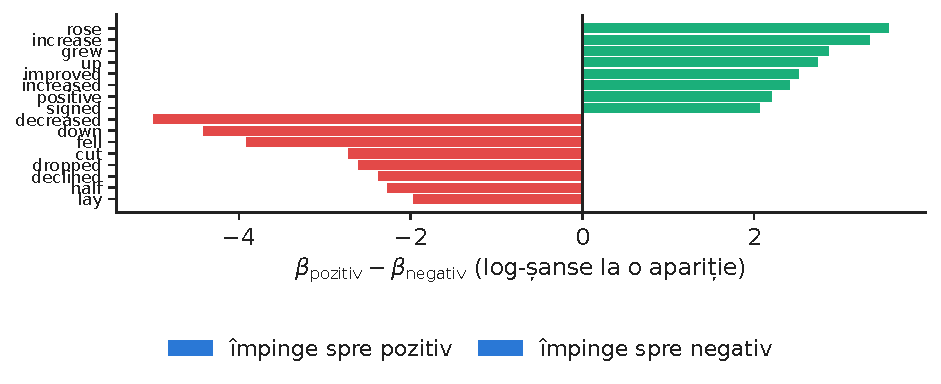
\includegraphics[width=\textwidth,height=0.319\textheight,keepaspectratio]{charts/ro/top_words.pdf}\end{center}\vspace{-3mm}
\chartsource{Sursa: Financial PhraseBank (Malo et al., 2014). Date: 4.838 de fraze din știri financiare, 5-8 adnotatori pentru fiecare.}
\vspace{0.5mm}
\begin{itemize}\setlength{\itemsep}{0pt}
  \item Cele mai pozitive: rose, increase, grew, up, improved
    \begin{itemize}\setlength{\itemsep}{0pt}
      \item Cele mai negative: decreased, down, fell, cut, dropped.
    \end{itemize}
  \item Dicționarele de limbaj general interpretează greșit cuvintele financiare (``liability'', ``tax''): învățați ponderile pe texte financiare.
\end{itemize}
\par\vfill\noindent{\scriptsize\color{FooterGray}(Loughran \& McDonald, 2011; calcul propriu)}\hfill\qlink{NN\_L6\_top\_words}{Quantlets/L6/NN_L6_top_words}\par\vspace{0.5mm}
\end{frame}


\section{Reprezentări dense: vectorii de cuvinte (embeddings)}

\begin{frame}{Un cuvînt se cunoaște după vecinii lui}
\footnotesize
\intuition{cuvintele folosite în contexte asemănătoare primesc vectori asemănători; asemănarea este cosinusul unghiului.}
\begin{columns}[T,onlytextwidth]
\begin{column}{0.53\textwidth}
\[ \mathbf e_w=\mathbf E^{\top}\mathbf o_w\in\R^{d},\qquad \cos(w,v)=\frac{\mathbf e_w^{\top}\mathbf e_v}{\|\mathbf e_w\|\,\|\mathbf e_v\|} \]{\footnotesize\begin{itemize}\setlength{\itemsep}{0pt}
  \item \textbf{\txtwhere}
    \begin{itemize}\setlength{\itemsep}{0pt}
      \item $\mathbf o_w\in\{0,1\}^{V}$ vectorul one-hot al cuvîntului $w$
      \item $\mathbf E\in\R^{V\times d}$ matricea vectorilor, $d=100\ll V=8\,539$
      \item În cod este o căutare, nu un produs
    \end{itemize}
\end{itemize}\par}
\end{column}
\begin{column}{0.44\textwidth}
\begin{itemize}\setlength{\itemsep}{2pt}
  \item Vectorii one-hot sînt ortogonali: ``inflation'' și ``prices'' au cosinusul 0.
  \item În vectorii noștri: cos(inflation, prices) = 0{,}49, cos(inflation, climate) = 0{,}16, cos(banks, lending) = 0{,}46.
\end{itemize}
\end{column}
\end{columns}
\par\vfill\manager{vectorii denși permit unui model antrenat pe ``profit rose'' să generalizeze la ``earnings increased''.}\par\vspace{0.5mm}
\par\vfill\noindent{\scriptsize\color{FooterGray}(Firth, 1957; Bishop \& Bishop, 2024, secț.~12.2)}\par\vspace{0.5mm}
\end{frame}

\begin{frame}{word2vec skip-gram: prezicem contextul din cuvînt}
\footnotesize
\intuition{fiecare cuvînt din fereastra din jurul cuvîntului central este prezis printr-un softmax peste vocabular.}
\begin{columns}[T,onlytextwidth]
\begin{column}{0.6\textwidth}
\[ \max_{\mathbf U,\mathbf V}\;\frac1T\sum_{t=1}^{T}\sum_{0<|j|\le c}\log p(w_{t+j}\mid w_t) \]\vspace{-2mm}\[ p(o\mid w)=\frac{\exp(\mathbf u_o^{\top}\mathbf v_w)}{\sum_{k=1}^{V}\exp(\mathbf u_k^{\top}\mathbf v_w)} \]{\footnotesize\begin{itemize}\setlength{\itemsep}{0pt}
  \item \textbf{\txtwhere}
    \begin{itemize}\setlength{\itemsep}{0pt}
      \item $\mathbf v_w$ vectorul de intrare (al cuvîntului central)
      \item $\mathbf u_o$ vectorul de ieșire (al contextului)
      \item $c$ raza ferestrei
      \item Numitorul costă $O(V)$ pentru fiecare pereche
    \end{itemize}
\end{itemize}\par}
\end{column}
\begin{column}{0.37\textwidth}
\begin{itemize}\setlength{\itemsep}{2pt}
  \item Sacul continuu de cuvinte (CBOW) este varianta în oglindă: prezice cuvîntul central din media contextului.
  \item Rețea liniară cu un strat ascuns
    \begin{itemize}\setlength{\itemsep}{0pt}
      \item Vectorii de cuvinte sînt prima ei matrice de ponderi.
    \end{itemize}
  \item Corpusul nostru: 3\,679\,754 de perechi (cuvînt central, context) pe epocă, după subeșantionare.
\end{itemize}
\end{column}
\end{columns}
\par\vfill\manager{softmax-ul peste 8\,539 de cuvinte este prea lent
    \begin{itemize}\setlength{\itemsep}{0pt}
      \item Îl înlocuim prin eșantionare negativă.
    \end{itemize}}\par\vspace{0.5mm}
\par\vfill\noindent{\scriptsize\color{FooterGray}(Mikolov et al., 2013)}\par\vspace{0.5mm}
\end{frame}

\begin{frame}{Eșantionarea negativă: deosebim perechile reale de cele aleatoare}
\footnotesize
\intuition{înlocuim softmax-ul cu $K+1$ regresii logistice binare: un cuvînt real de context și $K$ cuvinte de zgomot.}
\begin{columns}[T,onlytextwidth]
\begin{column}{0.53\textwidth}
\[ \ell(w,o)=-\log\sigma(\mathbf u_o^{\top}\mathbf v_w)-\sum_{k=1}^{K}\log\sigma(-\mathbf u_{n_k}^{\top}\mathbf v_w) \]\vspace{-2mm}\[ n_k\sim P_n(w)\propto f(w)^{3/4} \]{\footnotesize\begin{itemize}\setlength{\itemsep}{0pt}
  \item \textbf{\txtwhere}
    \begin{itemize}\setlength{\itemsep}{0pt}
      \item $\sigma$ funcția logistică
      \item $K=5$
      \item $f(w)$ frecvența în corpus
      \item Cuvintele frecvente sînt păstrate cu probabilitatea $\min(1,\sqrt{t/f(w)}+t/f(w))$, $t=10^{-4}$
    \end{itemize}
\end{itemize}\par}
\end{column}
\begin{column}{0.44\textwidth}
\begin{itemize}\setlength{\itemsep}{2pt}
  \item Skip-gram cu eșantionare negativă (SGNS), $d=100$, fereastră 5, cuvinte cu cel puțin 5 apariții, Adam, 5 epoci în 120 de secunde.
  \item Pierderea pe pereche scade de la 2{,}622 (epoca 1) la 2{,}223.
  \item SGNS factorizează implicit o matrice deplasată de informație mutuală punctuală (PMI) (anexă).
\end{itemize}
\end{column}
\end{columns}
\par\vfill\manager{același truc, contrastul dintre un element real și negative eșantionate, antrenează sisteme de recomandare și reprezentări pentru detectarea fraudei.}\par\vspace{0.5mm}
\par\vfill\noindent{\scriptsize\color{FooterGray}(Mikolov et al., 2013; Levy \& Goldberg, 2014)}\par\vspace{0.5mm}
\end{frame}

\begin{frame}{GloVe: aproximăm logaritmul frecvențelor de co-apariție}
\footnotesize
\intuition{numărăm o singură dată cît de des apar cuvintele împreună, apoi aproximăm logaritmii acestor frecvențe prin produse scalare, cu o pierdere de tip cele mai mici pătrate ponderate.}
\begin{columns}[T,onlytextwidth]
\begin{column}{0.5\textwidth}
\[ J=\sum_{i,j:\,X_{ij}>0}f(X_{ij})\big(\mathbf w_i^{\top}\tilde{\mathbf w}_j+b_i+\tilde b_j-\ln X_{ij}\big)^2 \]\vspace{-2mm}\[ f(x)=\min\{1,(x/x_{\max})^{\alpha}\} \]{\footnotesize\begin{itemize}\setlength{\itemsep}{0pt}
  \item \textbf{\txtwhere}
    \begin{itemize}\setlength{\itemsep}{0pt}
      \item $X_{ij}$ co-aparițiile la cel mult 10 cuvinte distanță, ponderate cu $1/\text{distanță}$
      \item $x_{\max}=100$, $\alpha=0{,}75$
      \item Vectorul final este $\mathbf w_i+\tilde{\mathbf w}_i$
    \end{itemize}
\end{itemize}\par}
\end{column}
\begin{column}{0.47\textwidth}
\begin{center}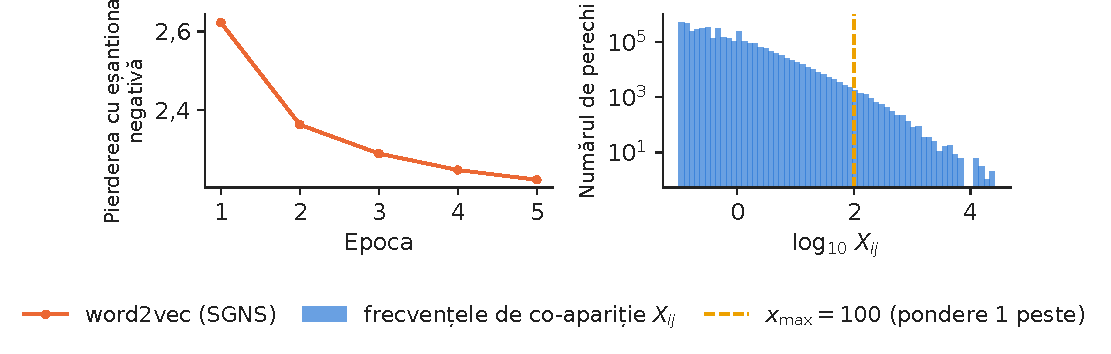
\includegraphics[width=\textwidth,height=0.500\textheight,keepaspectratio]{charts/ro/emb_training.pdf}\end{center}\vspace{-3mm}
\chartsource{Sursa: Banca Centrală Europeană, setul de discursuri. Date: 8 ianuarie 2022 - 30 octombrie 2026, 400 de discursuri.}
\end{column}
\end{columns}
\par\vfill\manager{3\,841\,517 de perechi nenule (5{,}269\,\% din $V^2$)
    \begin{itemize}\setlength{\itemsep}{0pt}
      \item 99{,}81\,\% sînt sub $x_{\max}$ și primesc o pondere sub 1.
    \end{itemize}}\par\vspace{0.5mm}
\par\vfill\noindent{\scriptsize\color{FooterGray}(Pennington et al., 2014; calcul propriu)}\hfill\qlink{NN\_L6\_emb\_training}{Quantlets/L6/NN_L6_emb_training}\par\vspace{0.5mm}
\end{frame}

\begin{frame}{Numărarea este suficientă: PMI și o factorizare trunchiată}
\footnotesize
\intuition{înaintea vectorilor neuronali, vectorii denși proveneau din factorizarea unei matrice de asocieri între cuvinte.}
\begin{columns}[T,onlytextwidth]
\begin{column}{0.6\textwidth}
\[ \mathrm{PMI}(w,c)=\ln\frac{P(w,c)}{P(w)P(c)} \]\vspace{-2mm}\[ \mathbf M_{+}\approx\mathbf U_d\boldsymbol\Sigma_d\mathbf V_d^{\top},\qquad \mathbf E=\mathbf U_d\boldsymbol\Sigma_d^{1/2} \]{\footnotesize\begin{itemize}\setlength{\itemsep}{0pt}
  \item \textbf{\txtwhere}
    \begin{itemize}\setlength{\itemsep}{0pt}
      \item $P(w,c)$ ponderea co-aparițiilor lui $w$ și $c$
      \item $\mathbf M_{+}$ matricea valorilor $\max(\mathrm{PMI},0)$
      \item $\mathbf U_d,\boldsymbol\Sigma_d,\mathbf V_d$ primii $d$ termeni ai descompunerii în valori singulare (SVD)
    \end{itemize}
\end{itemize}\par}
\end{column}
\begin{column}{0.37\textwidth}
\begin{itemize}\setlength{\itemsep}{2pt}
  \item Informația mutuală punctuală (PMI) este pozitivă cînd două cuvinte apar împreună mai des decît la întîmplare.
  \item Tabelul nostru de co-apariții are 3\,841\,517 de perechi nenule, 5{,}269\,\% din cele $V^2$ celule: o matrice rară, deci SVD este ieftin.
  \item word2vec, GloVe și SVD-ul matricei PMI dau vecini asemănători pe același corpus.
\end{itemize}
\end{column}
\end{columns}
\par\vfill\manager{o factorizare a frecvențelor este transparentă și reproductibilă: un prim vector de cuvinte bun pentru un corpus intern.}\par\vspace{0.5mm}
\par\vfill\noindent{\scriptsize\color{FooterGray}(Levy \& Goldberg, 2014)}\par\vspace{0.5mm}
\end{frame}

\begin{frame}{Cei mai apropiați vecini în vectorii noștri, învățați din discursurile băncii centrale}
\footnotesize
{\scriptsize\renewcommand{\arraystretch}{1.05}\setlength{\tabcolsep}{4pt}
\begin{tabular}{@{}p{0.13\textwidth}p{0.4\textwidth}p{0.4\textwidth}@{}}\toprule
Cuvîntul & word2vec (SGNS) & GloVe \\ \midrule
\texttt{inflation} & headline, underlying, revert, hovering, medium & expectations, underlying, headline, core, term \\
\texttt{energy} & fertilisers, food, hicpxx, prices, renewable & prices, food, shock, commodity, renewable \\
\texttt{banks} & repaying, supervisors, themselves, obtaining, supervised & central, their, supervisors, they, have \\
\texttt{climate} & change, environmental, degradation, nature, ipcc & change, nature, environmental, related, risks \\
\texttt{digital} & convenient, functionality, kantar, erpb, payments & euro, payments, form, would, cash \\
\texttt{wages} & wage, profits, catch, negotiated, salaries & real, nominal, higher, incomes, rising \\
\texttt{ukraine} & invasion, russia, aggression, russian, brutal & invasion, russia, war, unjustified, russian \\
\texttt{rates} & interest, rate, compressed, hikes, repriced & interest, rate, short, lending, long \\
\bottomrule\end{tabular}}
\par\vspace{0.5mm}{\scriptsize \begin{itemize}\setlength{\itemsep}{0pt}
  \item Cele mai apropiate cinci cuvinte după cosinus; ambele modele sînt antrenate pe aceleași 1\,289\,896 de unități lexicale din discursurile BCE; suprapunerea medie a celor două liste: 1{,}88 cuvinte.
\end{itemize}}
\par\vfill\manager{un analist al politicii monetare poate extinde o căutare după ``inflation'' cu vecinii învățați, în locul unei liste făcute de mînă.}\par\vspace{0.5mm}
\par\vfill\noindent{\scriptsize\color{FooterGray}(calcul propriu)}\hfill\tryit{\S2}\par\vspace{0.5mm}
\end{frame}

\begin{frame}{Temele activității băncii centrale formează regiuni în spațiul vectorilor}
\small
\intuition{proiecția bidimensională prin analiza componentelor principale (PCA) a 32 de cuvinte alese din patru grupuri; grupurile nu au fost date modelului.}
\begin{center}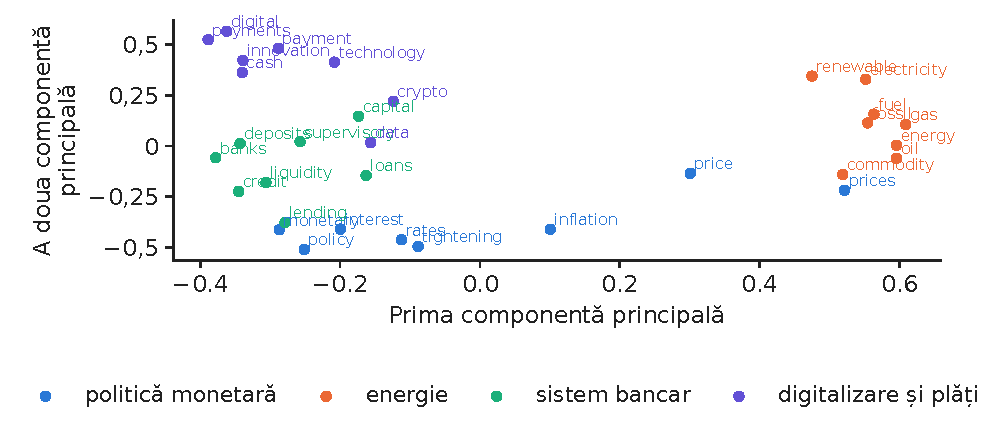
\includegraphics[width=\textwidth,height=0.500\textheight,keepaspectratio]{charts/ro/w2v_pca.pdf}\end{center}\vspace{-3mm}
\chartsource{Sursa: Banca Centrală Europeană, setul de discursuri. Date: 8 ianuarie 2022 - 30 octombrie 2026, 400 de discursuri.}
\vspace{0.5mm}
\begin{itemize}\setlength{\itemsep}{0pt}
  \item Două componente păstrează 31{,}9\,\% din varianța acestor 32 de vectori, deci imaginea este doar o umbră aproximativă a spațiului $\R^{100}$.
\end{itemize}
\par\vfill\noindent{\scriptsize\color{FooterGray}(calcul propriu)}\hfill\qlink{NN\_L6\_w2v\_pca}{Quantlets/L6/NN_L6_w2v_pca}\par\vspace{0.5mm}
\end{frame}

\begin{frame}{Analogii și limitele unui singur vector pentru fiecare cuvînt}
\footnotesize
\begin{columns}[T,onlytextwidth]
\begin{column}{0.46\textwidth}
{\scriptsize\renewcommand{\arraystretch}{1.05}\setlength{\tabcolsep}{4pt}
\begin{tabular}{@{}ll@{}}\toprule
$a:b::c:\,?$ & răspuns \\ \midrule
\texttt{germany : german : : france} & \texttt{fran} \\
\texttt{italy : italian : : spain} & \texttt{commissioned} \\
\texttt{banks : bank : : households} & \texttt{household} \\
\texttt{rise : rising : : fall} & \texttt{buffered} \\
\texttt{higher : lower : : increase} & \texttt{marginal} \\
\bottomrule\end{tabular}}
\par\vspace{0.5mm}{\scriptsize \begin{itemize}\setlength{\itemsep}{0pt}
  \item Răspunsul $=\argmax_v\cos(\mathbf e_v,\mathbf e_b-\mathbf e_a+\mathbf e_c)$, excluzînd $a,b,c$; word2vec-ul nostru, un singur corpus mic.
\end{itemize}}
\end{column}
\begin{column}{0.51\textwidth}
\begin{itemize}\setlength{\itemsep}{4pt}
  \item \textbf{Vectori statici}
    \begin{itemize}\setlength{\itemsep}{0pt}
      \item Un singur vector pentru fiecare cuvînt, indiferent de frază
      \item ``interest'' (dobîndă) și ``interest'' (atenție) au același vector; la fel ``bank''
    \end{itemize}
  \item \textbf{Acoperirea}
    \begin{itemize}\setlength{\itemsep}{0pt}
      \item Vocabularul BCE acoperă 84{,}7\,\% din unitățile lexicale din PhraseBank și 76{,}4\,\% din cele din tweet-uri
      \item Restul sînt în afara vocabularului (OOV); modelele cu subcuvinte (fastText) și transformerele (cursul 7) rezolvă ambele probleme
    \end{itemize}
\end{itemize}
\end{column}
\end{columns}
\par\vfill\noindent{\scriptsize\color{FooterGray}(Mikolov et al., 2013; Bojanowski et al., 2017)}\par\vspace{0.5mm}
\end{frame}

\begin{frame}{Vectori din subcuvinte pentru cuvintele nevăzute}
\footnotesize
\intuition{construim vectorul unui cuvînt din vectorii $n$-gramelor sale de caractere, astfel încît un simbol bursier nou sau o greșeală de scriere primește totuși un vector.}
\begin{columns}[T,onlytextwidth]
\begin{column}{0.53\textwidth}
\[ \mathbf e_w=\sum_{g\in\mathcal G(w)}\mathbf z_g \]{\footnotesize\begin{itemize}\setlength{\itemsep}{0pt}
  \item \textbf{\txtwhere}
    \begin{itemize}\setlength{\itemsep}{0pt}
      \item $\mathcal G(w)$ $n$-gramele de caractere ale lui $w$ (de exemplu de 3--6 caractere, cu simboluri de margine) și cuvîntul însuși
      \item $\mathbf z_g$ vectori învățați ai $n$-gramelor
    \end{itemize}
\end{itemize}\par}
\end{column}
\begin{column}{0.44\textwidth}
\begin{itemize}\setlength{\itemsep}{2pt}
  \item Acoperirea vocabularului nostru BCE la nivel de cuvînt: 84{,}7\,\% din unitățile lexicale PhraseBank, 76{,}4\,\% din cele din tweet-uri.
  \item Modelele cu subcuvinte (fastText) împart informația între ``profit'', ``profits'' și ``profitability''.
  \item Transformerele (cursul 7) folosesc aceeași idee, cu unități de subcuvinte învățate.
\end{itemize}
\end{column}
\end{columns}
\par\vfill\manager{pentru tweet-uri și mesaje, cu simboluri bursiere și variante de scriere, folosiți vectori din subcuvinte sau un tokenizator pe subcuvinte.}\par\vspace{0.5mm}
\par\vfill\noindent{\scriptsize\color{FooterGray}(Bojanowski et al., 2017)}\par\vspace{0.5mm}
\end{frame}


\section{Clasificatoare de fraze: reprezentări rare și dense}

\begin{frame}{O rețea embedding bag: media vectorilor de cuvinte, apoi un softmax}
\footnotesize
\intuition{cel mai simplu clasificator neuronal de text învață împreună vectorii de cuvinte și clasificatorul.}
\begin{columns}[T,onlytextwidth]
\begin{column}{0.53\textwidth}
\[ \mathbf z=\frac{1}{|S|}\sum_{s\in S}\mathbf e_s \]\vspace{-2mm}\[ \hat{\mathbf p}=\softmax(\mW\,\mathrm{dropout}(\mathbf z)+\vb) \]\vspace{-2mm}\[ \loss=-\frac1n\sum_i\omega_{y_i}\log\hat p_{i,y_i} \]{\footnotesize\begin{itemize}\setlength{\itemsep}{0pt}
  \item \textbf{\txtwhere}
    \begin{itemize}\setlength{\itemsep}{0pt}
      \item $S$ unitățile lexicale și bigramele frazei
      \item $\mathbf e_s$ vectori învățați ($d=100$)
      \item $\omega_k=n/(3n_k)$ ponderi ale claselor, împotriva dominanței clasei ``neutru''
    \end{itemize}
\end{itemize}\par}
\end{column}
\begin{column}{0.44\textwidth}
\begin{itemize}\setlength{\itemsep}{2pt}
  \item Start aleator sau start word2vec: rîndurile lui $\mathbf E$ sînt inițializate cu vectorii noștri BCE, apoi ajustate.
  \item Comparăm și: media vectorilor word2vec + regresie logistică (vectori înghețați), TF-IDF + un perceptron multistrat (MLP) cu 128 de unități ascunse.
\end{itemize}
\end{column}
\end{columns}
\par\vfill\manager{aceasta este arhitectura clasificatoarelor de tip fastText, folosite în producție pentru milioane de documente pe oră.}\par\vspace{0.5mm}
\par\vfill\noindent{\scriptsize\color{FooterGray}(Joulin et al., 2017)}\par\vspace{0.5mm}
\end{frame}

\begin{frame}{Regresia logistică pe text: gradientul}
\footnotesize
\intuition{modelul logistic multinomial este o rețea cu un singur strat; gradientul lui compară probabilitățile prezise cu clasele reale.}
\begin{columns}[T,onlytextwidth]
\begin{column}{0.53\textwidth}
\[ \loss(\mathbf B)=-\sum_{i}\sum_k y_{ik}\ln\hat p_{ik}+\frac{1}{2C}\|\mathbf B\|_F^2 \]\vspace{-2mm}\[ \nabla_{\mathbf B}\loss=\mathbf X^{\top}(\hat{\mathbf P}-\mathbf Y)+\mathbf B/C \]{\footnotesize\begin{itemize}\setlength{\itemsep}{0pt}
  \item \textbf{\txtwhere}
    \begin{itemize}\setlength{\itemsep}{0pt}
      \item $\mathbf X$ matricea TF-IDF ($n\times V$, rară)
      \item $\mathbf Y$ etichetele one-hot
      \item $\hat{\mathbf P}$ probabilitățile softmax
      \item $C$ inversul penalizării, ales pe validare din $\{0{,}1;1;10\}$
    \end{itemize}
\end{itemize}\par}
\end{column}
\begin{column}{0.44\textwidth}
\begin{itemize}\setlength{\itemsep}{2pt}
  \item Pierdere convexă: un singur optim, fără sămînță de raportat
    \begin{itemize}\setlength{\itemsep}{0pt}
      \item Perceptronul multistrat (MLP) pe aceleași intrări adaugă un strat ascuns de 128 de unități.
    \end{itemize}
  \item Macro-F1 pe PhraseBank: logistic 73{,}49\,\%, MLP 71{,}37\,\%: stratul ascuns nu ajută aici.
\end{itemize}
\end{column}
\end{columns}
\par\vfill\manager{cu cîteva mii de fraze scurte, flexibilitatea suplimentară a unei rețele aduce varianță, nu acuratețe.}\par\vspace{0.5mm}
\par\vfill\noindent{\scriptsize\color{FooterGray}(calcul propriu)}\par\vspace{0.5mm}
\end{frame}

\begin{frame}{De la vectorii cuvintelor la vectorul frazei}
\footnotesize
\intuition{media vectorilor de cuvinte este cea mai simplă reprezentare a unei fraze și pierde exact ce contează pentru sentiment.}
\begin{columns}[T,onlytextwidth]
\begin{column}{0.53\textwidth}
\[ \mathbf s_i=\frac{1}{|S_i|}\sum_{w\in S_i}\mathbf e_w,\qquad \mathbf s_i^{\mathrm{w}}=\frac{\sum_{w}a_w\mathbf e_w}{\sum_w a_w},\ \ a_w=\frac{\alpha}{\alpha+f(w)} \]{\footnotesize\begin{itemize}\setlength{\itemsep}{0pt}
  \item \textbf{\txtwhere}
    \begin{itemize}\setlength{\itemsep}{0pt}
      \item $S_i$ unitățile lexicale din vocabular ale frazei $i$
      \item $a_w$ o pondere care micșorează influența cuvintelor frecvente
      \item $\alpha$ o constantă mică
    \end{itemize}
\end{itemize}\par}
\end{column}
\begin{column}{0.44\textwidth}
\begin{itemize}\setlength{\itemsep}{2pt}
  \item Media vectorilor BCE înghețați + regresie logistică: macro-F1 57{,}30\,\% pe PhraseBank și 53{,}71\,\% pe tweet-uri.
  \item ``rose'' și ``fell'' sînt apropiate într-un spațiu de co-apariții (aceleași contexte), deci media estompează semnul.
  \item Ajustarea vectorilor pe date etichetate (embedding bag) recuperează cea mai mare parte a diferenței.
\end{itemize}
\end{column}
\end{columns}
\par\vfill\manager{vectorii generali sînt buni pentru căutare și similaritate, nu în mod automat pentru sentiment.}\par\vspace{0.5mm}
\par\vfill\noindent{\scriptsize\color{FooterGray}(calcul propriu)}\par\vspace{0.5mm}
\end{frame}

\begin{frame}{Protocolul și metrica: macro-F1 pentru o țintă dezechilibrată}
\footnotesize
\intuition{clasa ``neutru'' reprezintă 59{,}3\,\% din PhraseBank, deci acuratețea răsplătește un model care spune mereu ``neutru''.}
\begin{columns}[T,onlytextwidth]
\begin{column}{0.53\textwidth}
\[ \mathrm{F1}_k=\frac{2P_kR_k}{P_k+R_k},\qquad \text{macro-F1}=\frac13\sum_{k=1}^{3}\mathrm{F1}_k \]{\footnotesize\begin{itemize}\setlength{\itemsep}{0pt}
  \item \textbf{\txtwhere}
    \begin{itemize}\setlength{\itemsep}{0pt}
      \item $P_k$ precizia și $R_k$ sensibilitatea clasei $k$
      \item Fiecare clasă contează la fel, indiferent de mărime
    \end{itemize}
\end{itemize}\par}
\end{column}
\begin{column}{0.44\textwidth}
\begin{itemize}\setlength{\itemsep}{2pt}
  \item PhraseBank: 5 împărțiri aleatoare stratificate 70/15/15
    \begin{itemize}\setlength{\itemsep}{0pt}
      \item Tweet-uri: setul de validare publicat, folosit ca test, 3 semințe.
    \end{itemize}
  \item Penalizarea $C$, oprirea timpurie și vocabularul sînt alese numai pe partea de validare.
\end{itemize}
\end{column}
\end{columns}
\par\vfill\manager{pentru un sistem de alertă, raportați sensibilitatea clasei negative alături de macro-F1: aceasta este clasa care costă bani.}\par\vspace{0.5mm}
\par\vfill\noindent{\scriptsize\color{FooterGray}(calcul propriu)}\hfill\tryit{\S3}\par\vspace{0.5mm}
\end{frame}

\begin{frame}{Pe frazele financiare scurte, TF-IDF este greu de depășit}
\small
\intuition{macro-F1 pe test pentru șapte reprezentări și clasificatoare, PhraseBank și tweet-uri financiare (bare: media, mustăți: abaterea standard).}
\begin{center}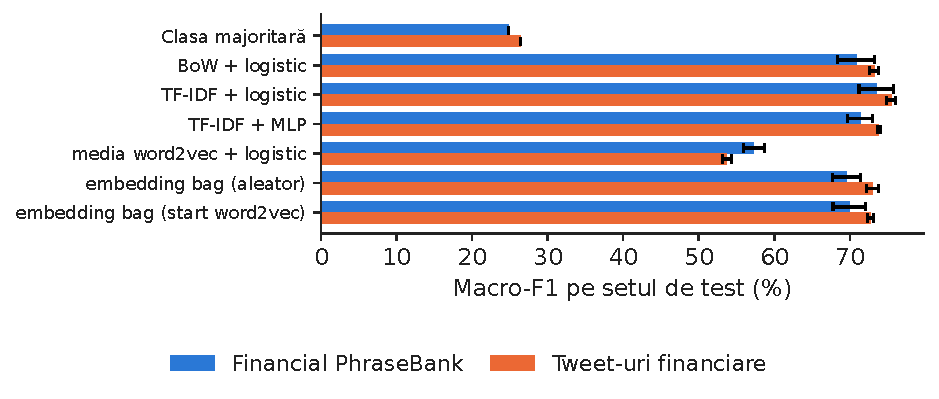
\includegraphics[width=\textwidth,height=0.470\textheight,keepaspectratio]{charts/ro/sentiment_models.pdf}\end{center}\vspace{-3mm}
\chartsource{Sursa: Financial PhraseBank (Malo et al., 2014); Twitter financial news (Hugging Face, zeroshot). Date: PhraseBank: 5 împărțiri aleatoare 70/15/15; tweet-uri: setul de validare publicat, folosit ca test, 3 semințe.}
\vspace{0.5mm}
\begin{itemize}\setlength{\itemsep}{0pt}
  \item Pe PhraseBank: 73{,}49 (TF-IDF + logistic), față de 69{,}93 (embedding bag, start word2vec)
    \begin{itemize}\setlength{\itemsep}{0pt}
      \item Clasa majoritară 24{,}81.
    \end{itemize}
\end{itemize}
\par\vfill\noindent{\scriptsize\color{FooterGray}(calcul propriu)}\hfill\qlink{NN\_L6\_sentiment\_models}{Quantlets/L6/NN_L6_sentiment_models}\par\vspace{0.5mm}
\end{frame}

\begin{frame}{Rezultatele pentru sentiment, cu incertitudine}
\footnotesize
{\scriptsize\renewcommand{\arraystretch}{1.05}\setlength{\tabcolsep}{4pt}
\begin{tabular}{@{}lrrrr@{}}\toprule
Modelul & PhraseBank macro-F1 & acur. & Tweet-uri macro-F1 & acur. \\ \midrule
Clasa majoritară & 24{,}81\,$\pm$\,0{,}00 & 59{,}28 & 26{,}40\,$\pm$\,0{,}00 & 65{,}58 \\
BoW + logistic & 70{,}82\,$\pm$\,2{,}41 & 74{,}94 & 73{,}25\,$\pm$\,0{,}59 & 80{,}00 \\
TF-IDF + logistic & 73{,}49\,$\pm$\,2{,}28 & 77{,}69 & 75{,}47\,$\pm$\,0{,}56 & 81{,}77 \\
TF-IDF + MLP & 71{,}37\,$\pm$\,1{,}65 & 76{,}23 & 73{,}85\,$\pm$\,0{,}24 & 80{,}56 \\
media word2vec + logistic & 57{,}30\,$\pm$\,1{,}39 & 62{,}01 & 53{,}71\,$\pm$\,0{,}60 & 61{,}59 \\
embedding bag, start aleator & 69{,}56\,$\pm$\,1{,}81 & 74{,}11 & 72{,}97\,$\pm$\,0{,}78 & 79{,}77 \\
embedding bag, start word2vec & 69{,}93\,$\pm$\,2{,}16 & 74{,}99 & 72{,}76\,$\pm$\,0{,}39 & 79{,}51 \\
\bottomrule\end{tabular}}
\par\vspace{0.5mm}{\scriptsize \begin{itemize}\setlength{\itemsep}{0pt}
  \item Pereche, pe cele 5 împărțiri PhraseBank: TF-IDF + logistic minus embedding bag (start word2vec) $=\ensuremath{+}3{,}55$ puncte, $t=9{,}88$ (4 grade de libertate).
  \item Pornirea de la vectorii noștri word2vec BCE schimbă rezultatul embedding bag cu \ensuremath{+}0{,}37 puncte pe PhraseBank și cu \ensuremath{-}0{,}21 pe tweet-uri.
\end{itemize}}
\par\vfill\manager{modelul cel mai ieftin aflat la cel mult o abatere standard de cel mai bun este cel care trebuie folosit și explicat.}\par\vspace{0.5mm}
\par\vfill\noindent{\scriptsize\color{FooterGray}(calcul propriu)}\par\vspace{0.5mm}
\end{frame}

\begin{frame}{Cît de mare trebuie să fie vectorul de cuvinte?}
\footnotesize
\begin{columns}[T,onlytextwidth]
\begin{column}{0.35\textwidth}
{\footnotesize\renewcommand{\arraystretch}{1.05}\setlength{\tabcolsep}{4pt}
\begin{tabular}{@{}rr@{}}\toprule
Dimensiunea $d$ & Macro-F1 (\%) \\ \midrule
8 & 67{,}3 \\
16 & 66{,}5 \\
32 & 67{,}2 \\
64 & 67{,}8 \\
128 & 68{,}8 \\
256 & 67{,}3 \\
\bottomrule\end{tabular}}
\par\vspace{0.5mm}{\scriptsize \begin{itemize}\setlength{\itemsep}{0pt}
  \item Embedding bag, start aleator, împărțirea 1 PhraseBank, media pe 3 semințe.
\end{itemize}}
\end{column}
\begin{column}{0.62\textwidth}
\begin{itemize}\setlength{\itemsep}{4pt}
  \item Parametrii stratului de embedding: $V\times d$
    \begin{itemize}\setlength{\itemsep}{0pt}
      \item Cu bigrame, $V$ are cîteva mii de elemente, deci $d$ determină mărimea modelului.
    \end{itemize}
  \item Aici scorul variază puțin cu $d$: de la 67{,}3 la $d=8$ la 68{,}8 la $d=128$.
  \item O sarcină cu trei clase pe fraze scurte are nevoie de puține dimensiuni
    \begin{itemize}\setlength{\itemsep}{0pt}
      \item Vectorii de uz general folosesc 100--300 pentru că servesc multor sarcini.
    \end{itemize}
\end{itemize}
\end{column}
\end{columns}
\par\vfill\manager{alegeți $d$ pe datele de validare
    \begin{itemize}\setlength{\itemsep}{0pt}
      \item Un model mai mic este mai ieftin de rulat și de explicat.
    \end{itemize}}\par\vspace{0.5mm}
\par\vfill\noindent{\scriptsize\color{FooterGray}(calcul propriu)}\par\vspace{0.5mm}
\end{frame}

\begin{frame}{Modelele greșesc acolo unde adnotatorii nu sînt de acord}
\small
\intuition{acuratețea pe test în funcție de ponderea adnotatorilor care au fost de acord asupra etichetei frazei.}
\begin{center}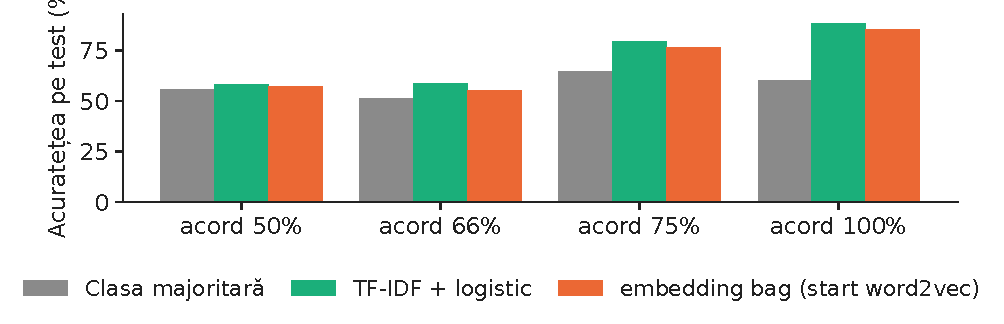
\includegraphics[width=\textwidth,height=0.349\textheight,keepaspectratio]{charts/ro/agreement.pdf}\end{center}\vspace{-3mm}
\chartsource{Sursa: Financial PhraseBank (Malo et al., 2014). Date: frazele de test din 5 împărțiri aleatoare, după ponderea adnotatorilor care sînt de acord.}
\vspace{0.5mm}
\begin{itemize}\setlength{\itemsep}{0pt}
  \item TF-IDF + logistic: 88{,}4\,\% pe frazele cu acord unanim, 58{,}1\,\% la un acord de 50\,\%
    \begin{itemize}\setlength{\itemsep}{0pt}
      \item 2\,259 din 4\,838 de fraze au acord unanim.
    \end{itemize}
\end{itemize}
\par\vfill\manager{zgomotul din etichete limitează orice model: înainte de a cumpăra un model mai mare, verificați cît de mult sînt de acord propriii analiști.}\par\vspace{0.5mm}
\par\vfill\noindent{\scriptsize\color{FooterGray}(calcul propriu)}\hfill\qlink{NN\_L6\_agreement}{Quantlets/L6/NN_L6_agreement}\par\vspace{0.5mm}
\end{frame}

\begin{frame}{Cu puține etichete, startul word2vec ajută rețeaua; TF-IDF rămîne competitiv}
\small
\intuition{stînga: macro-F1 pe test în funcție de numărul de fraze etichetate; dreapta: dimensiunea vectorilor din embedding bag.}
\begin{center}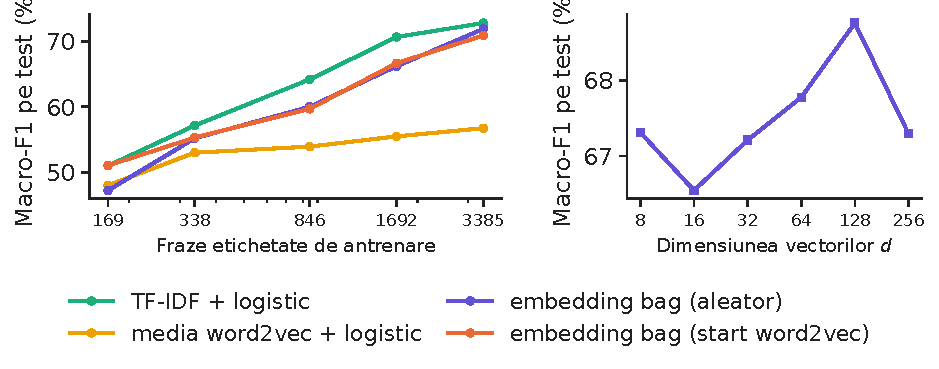
\includegraphics[width=\textwidth,height=0.420\textheight,keepaspectratio]{charts/ro/learning_curve.pdf}\end{center}\vspace{-3mm}
\chartsource{Sursa: Financial PhraseBank (Malo et al., 2014). Date: stînga: 3 împărțiri aleatoare; dreapta: embedding bag (start aleator), împărțirea 1, 3 semințe.}
\vspace{0.5mm}
\begin{itemize}\setlength{\itemsep}{0pt}
  \item Cu 169 de fraze etichetate: TF-IDF 51{,}0, media word2vec 48{,}0, embedding bag aleator 47{,}2, start word2vec 51{,}0
    \begin{itemize}\setlength{\itemsep}{0pt}
      \item Cu toate cele 3\,385: 72{,}8, 56{,}7, 71{,}9, 70{,}9.
    \end{itemize}
\end{itemize}
\par\vfill\noindent{\scriptsize\color{FooterGray}(calcul propriu)}\hfill\qlink{NN\_L6\_learning\_curve}{Quantlets/L6/NN_L6_learning_curve}\par\vspace{0.5mm}
\end{frame}

\begin{frame}{Unde sînt erorile: știrile negative citite ca neutre}
\footnotesize
\begin{columns}[T,onlytextwidth]
\begin{column}{0.47\textwidth}
{\footnotesize\renewcommand{\arraystretch}{1.05}\setlength{\tabcolsep}{4pt}
\begin{tabular}{@{}lrrr@{}}\toprule
Real \textbackslash{} prezis & neg. & neu. & poz. \\ \midrule
negativ & -- & 107 & 48 \\
pozitiv & 50 & 263 & -- \\
\bottomrule\end{tabular}}
\par\vspace{0.5mm}{\scriptsize \begin{itemize}\setlength{\itemsep}{0pt}
  \item TF-IDF + logistic, cele 5 seturi de test PhraseBank reunite (3\,635 de fraze).
\end{itemize}}
\end{column}
\begin{column}{0.5\textwidth}
\begin{itemize}\setlength{\itemsep}{4pt}
  \item Sensibilitatea: negativ 65{,}9\,\%, neutru 84{,}1\,\%, pozitiv 69{,}5\,\%.
  \item Erorile de semn opus sînt rare
    \begin{itemize}\setlength{\itemsep}{0pt}
      \item Cele mai multe erori mută fraza în clasa neutră.
    \end{itemize}
  \item Eroare tipică: o scădere descrisă cu cuvinte neutre și cifre (``sales were EUR 10 mn, down from 12'').
\end{itemize}
\end{column}
\end{columns}
\par\vfill\manager{în finanțe, cifrele poartă sentiment
    \begin{itemize}\setlength{\itemsep}{0pt}
      \item Înlocuirea lor cu o singură unitate pierde comparațiile de tip ``down from'' pe care un model secvențial le poate citi.
    \end{itemize}}\par\vspace{0.5mm}
\par\vfill\noindent{\scriptsize\color{FooterGray}(calcul propriu)}\par\vspace{0.5mm}
\end{frame}


\section{Studiu de caz: temele tweet-urilor financiare}

\begin{frame}{Douăzeci de teme: ușor pentru rezultate și Fed, greu pentru știrile generale}
\small
\intuition{F1 pe fiecare temă, pentru cele 4\,117 de tweet-uri de test (setul de validare publicat).}
\begin{center}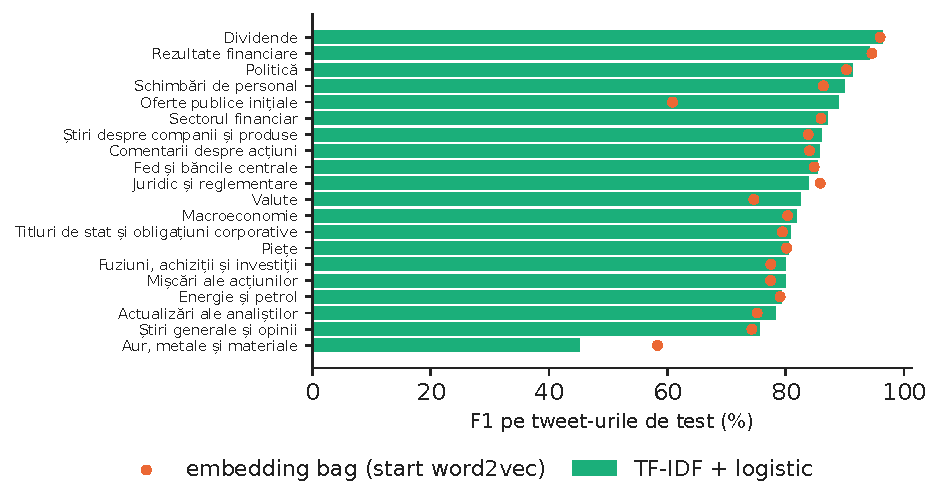
\includegraphics[width=\textwidth,height=0.525\textheight,keepaspectratio]{charts/ro/topic_f1.pdf}\end{center}\vspace{-3mm}
\chartsource{Sursa: Seturile Twitter financial news (Hugging Face, zeroshot). Date: 4.117 de tweet-uri de test (setul de validare publicat). 20 de teme.}
\vspace{0.5mm}
\begin{itemize}\setlength{\itemsep}{0pt}
  \item Macro-F1: TF-IDF + logistic 82{,}62\,\%, embedding bag (start word2vec) 80{,}45\,\%
    \begin{itemize}\setlength{\itemsep}{0pt}
      \item Acuratețe 84{,}48\,\%, față de 20{,}69\,\% pentru tema majoritară.
    \end{itemize}
\end{itemize}
\par\vfill\noindent{\scriptsize\color{FooterGray}(calcul propriu)}\hfill\qlink{NN\_L6\_topic\_f1}{Quantlets/L6/NN_L6_topic_f1}\par\vspace{0.5mm}
\end{frame}

\begin{frame}{Modele de text la lucru în finanțe}
\footnotesize
\begin{columns}[T,onlytextwidth]
\begin{column}{0.5\textwidth}
\begin{itemize}\setlength{\itemsep}{3pt}
  \item \textbf{Triajul știrilor și al tweet-urilor}
    \begin{itemize}\setlength{\itemsep}{0pt}
      \item Direcționarea pe teme (cea mai bună: Dividende, F1 96{,}4\,\%) și semnalarea celor negative pentru analist
    \end{itemize}
  \item \textbf{Comunicarea băncii centrale}
    \begin{itemize}\setlength{\itemsep}{0pt}
      \item Urmărirea cuvintelor din jurul lui ``inflation'' sau ``energy'', discurs cu discurs
    \end{itemize}
  \item \textbf{Conformitate și analiza de mediu, social și guvernanță (ESG)}
    \begin{itemize}\setlength{\itemsep}{0pt}
      \item Căutarea în rapoarte cu sinonime învățate, nu cu liste fixe de cuvinte-cheie
    \end{itemize}
\end{itemize}
\end{column}
\begin{column}{0.47\textwidth}
\begin{itemize}\setlength{\itemsep}{3pt}
  \item \textbf{Limitele modelelor de azi}
    \begin{itemize}\setlength{\itemsep}{0pt}
      \item Ordinea cuvintelor dincolo de bigrame se pierde
      \item Un singur vector pentru fiecare cuvînt ignoră contextul
      \item Tema cea mai slabă: Aur, metale și materiale, F1 45{,}2\,\%
    \end{itemize}
  \item \textbf{Urmează: atenția}
    \begin{itemize}\setlength{\itemsep}{0pt}
      \item Vectori contextuali din transformere, de exemplu reprezentări bidirecționale ale codificatorului transformer (BERT) și un model BERT adaptat textelor financiare (FinBERT), în cursul 7, comparați corect cu aceste modele de referință
    \end{itemize}
\end{itemize}
\end{column}
\end{columns}
\par\vfill\manager{începeți orice proiect de text cu TF-IDF + regresie logistică
    \begin{itemize}\setlength{\itemsep}{0pt}
      \item Treceți la vectori de cuvinte sau transformere doar cînd cîștigul este demonstrat pe datele dumneavoastră.
    \end{itemize}}\par\vspace{0.5mm}
\par\vfill\noindent{\scriptsize\color{FooterGray}(calcul propriu)}\par\vspace{0.5mm}
\end{frame}

\section*{Recapitulare}

\begin{frame}{Test 1: idf}
\small
\begin{itemize}
  \item Un cuvînt apare în fiecare dintre cele $n$ fraze de antrenare
    \begin{itemize}\setlength{\itemsep}{0pt}
      \item Care este idf-ul său netezit?
    \end{itemize}
\end{itemize}
\vspace{2mm}
\begin{exampleblock}{R\u{a}spuns}
\begin{itemize}
  \item $\ln\frac{1+n}{1+n}+1=1$: valoarea minimă, deci aproape nu modifică vectorul normalizat.
\end{itemize}
\end{exampleblock}
\end{frame}

\begin{frame}{Test 2: eșantionarea negativă}
\small
\begin{itemize}
  \item De ce extrage word2vec cuvintele negative din $f(w)^{3/4}$ și nu din $f(w)$?
\end{itemize}
\vspace{2mm}
\begin{exampleblock}{R\u{a}spuns}
\begin{itemize}
  \item Puterea 3/4 aplatizează distribuția: cuvintele rare sînt extrase mai des decît frecvența lor, iar cele frecvente, ca ``the'', mai rar, ceea ce dă contraste mai utile.
\end{itemize}
\end{exampleblock}
\end{frame}

\begin{frame}{Test 3: acuratețea}
\small
\begin{itemize}
  \item Un furnizor raportează o acuratețe de 60\,\% pe sentimentul din PhraseBank
    \begin{itemize}\setlength{\itemsep}{0pt}
      \item Este un rezultat bun?
    \end{itemize}
\end{itemize}
\vspace{2mm}
\begin{exampleblock}{R\u{a}spuns}
\begin{itemize}
  \item Nu: prognoza ``mereu neutru'' dă 59{,}28\,\%
    \begin{itemize}\setlength{\itemsep}{0pt}
      \item Cereți macro-F1 (TF-IDF + logistic, la noi: 73{,}49\,\%).
    \end{itemize}
\end{itemize}
\end{exampleblock}
\end{frame}

\begin{frame}{Test 4: transferul}
\small
\begin{itemize}
  \item Aveți doar 169 de fraze etichetate
    \begin{itemize}\setlength{\itemsep}{0pt}
      \item Ce reprezentare ajută cel mai mult?
    \end{itemize}
\end{itemize}
\vspace{2mm}
\begin{exampleblock}{R\u{a}spuns}
\begin{itemize}
  \item Comparați pe datele de validare: aici media word2vec dă 48{,}0, TF-IDF 51{,}0, embedding bag cu start word2vec 51{,}0 macro-F1.
\end{itemize}
\end{exampleblock}
\end{frame}

\begin{frame}{Test 5: polisemia}
\small
\begin{itemize}
  \item De ce nu poate un vector static să deosebească ``interest rate'' de ``of interest to investors''?
\end{itemize}
\vspace{2mm}
\begin{exampleblock}{R\u{a}spuns}
\begin{itemize}
  \item Are un singur vector pentru fiecare cuvînt, media tuturor utilizărilor lui
    \begin{itemize}\setlength{\itemsep}{0pt}
      \item Modelele contextuale (cursul 7) dau un vector diferit în fiecare frază.
    \end{itemize}
\end{itemize}
\end{exampleblock}
\end{frame}

\begin{frame}{Recapitulare}
\small
\vspace{-2mm}\begin{multicols}{2}\scriptsize\tableofcontents\end{multicols}
\begin{itemize}\setlength{\itemsep}{1pt}
  \item Textul devine numere prin unități lexicale și frecvențe (BoW, TF-IDF) sau prin vectori denși (word2vec, GloVe) învățați din co-apariții.
  \item Pe fraze financiare reale, TF-IDF + regresie logistică este modelul de depășit
    \begin{itemize}\setlength{\itemsep}{0pt}
      \item Startul word2vec ajută rețeaua doar cînd etichetele sînt puține
      \item Urmează atenția și transformerele (cursul 7).
    \end{itemize}
\end{itemize}
\end{frame}

\begin{frame}{Cercetări ale grupului nostru: modele de limbaj în finanțe}
\footnotesize
\begin{itemize}\setlength{\itemsep}{4pt}
  \item \textbf{Modelele lingvistice mari (LLM) prognozează valoarea expusă la risc (VaR) și pierderea medie peste VaR (ES)} (Pele, Bolovăneanu, Lin, Ren, Ginavar, Spilak, Andrei, Toma, Lessmann \& Härdle, 2026, Expert Systems with Applications)
    \begin{itemize}\setlength{\itemsep}{0pt}
      \item Lucrarea: ``In the beginning was the Word: LLM-VaR and LLM-ES''; prognozele LLM sînt comparate cu modelele clasice de risc prin teste retrospective formale
      \item Modelele de text trec de la scoruri de sentiment la cifrele de risc propriu-zise (cursul 12)
    \end{itemize}
  \item \textbf{BitMood: analiza cu inteligență artificială (AI) a tendințelor Bitcoin prin emoțiile de pe Facebook} (Conda, Găman, Bâg, Mazurencu-Marinescu-Pele, Pele \& Härdle, 2026, Digital Finance)
    \begin{itemize}\setlength{\itemsep}{0pt}
      \item 120.000 de postări de pe Facebook, 2015--2023, clasificate cu FinBERT în scoruri compuse de sentiment, împreună cu reacțiile cititorilor
      \item Sentimentul prognozează volumul tranzacțiilor cu Bitcoin; strategiile bazate pe sentiment depășesc strategia cumpără-și-păstrează; modelarea temelor urmărește subiectele discuției
    \end{itemize}
\end{itemize}
\par\vspace{0.5mm}{\scriptsize \begin{itemize}\setlength{\itemsep}{0pt}
  \item Rezultatele de pe acest diapozitiv sînt cele raportate în lucrări; celelalte cifre din curs provin din calculele noastre.
\end{itemize}}
\par\vfill\noindent{\scriptsize\color{FooterGray}(Academia de Studii Economice din București; Academia Română, Institutul de Prognoză Economică)}\par\vspace{0.5mm}
\end{frame}

\begin{frame}{Lecturi și resurse suplimentare}
\small
\begin{columns}[T,onlytextwidth]
\begin{column}{0.52\textwidth}
\begin{itemize}\setlength{\itemsep}{4pt}
  \item \textbf{Mikolov et al. (2013)} și \textbf{Pennington et al. (2014)}: cele două articole despre vectorii de cuvinte, ambele scurte.
  \item \textbf{Levy \& Goldberg (2014)}: de ce word2vec este o factorizare de matrice.
  \item \textbf{Loughran \& McDonald (2011)}: dicționarul de sentiment financiar și de ce eșuează dicționarele generale.
\end{itemize}
\end{column}
\begin{column}{0.45\textwidth}
\begin{itemize}\setlength{\itemsep}{4pt}
  \item \textbf{Acest curs}: cod, date, notebook-uri Jupyter --- \href{https://github.com/danpele/NEURAL_BIZ}{github.com/danpele/NEURAL\_BIZ}.
  \item \textbf{Exercițiu practic}: notebook-ul reproduce graficele acestui curs --- \href{\nnrepo/\nnnb}{notebooks/}.
  \item \textbf{Seminarul 6}: un indice de sentiment al discursurilor BCE, construit cu propriul clasificator.
\end{itemize}
\end{column}
\end{columns}
\end{frame}

\begin{frame}{Bibliografie (1/2)}
\scriptsize
\begin{itemize}\setlength{\itemsep}{0pt}\scriptsize
\item Bishop, C.\,M.\ \& Bishop, H.\ (2024). \textit{Deep Learning: Foundations and Concepts}, ch.~12. Springer. \href{https://doi.org/10.1007/978-3-031-45468-4}{doi:10.1007/978-3-031-45468-4}
\item Bojanowski, P., Grave, E., Joulin, A.\ \& Mikolov, T.\ (2017). Enriching word vectors with subword information. \textit{TACL}, 5, 135--146. \href{https://doi.org/10.1162/tacl_a_00051}{doi:10.1162/tacl\_a\_00051}
\item Conda, A.\,I., Găman, Ș., Bâg, R.\,C., Mazurencu-Marinescu-Pele, M., Pele, D.\,T.\ \& Härdle, W.\,K.\ (2026). BitMood: AI analysis of Bitcoin trends via Facebook emotions. \textit{Digital Finance}, 8(3), 42. \href{https://doi.org/10.1007/s42521-026-00205-3}{doi:10.1007/s42521-026-00205-3}
\item Firth, J.\,R.\ (1957). A synopsis of linguistic theory 1930--1955. In \textit{Studies in Linguistic Analysis}, 1--32. Blackwell.
\item Joulin, A., Grave, E., Bojanowski, P.\ \& Mikolov, T.\ (2017). Bag of tricks for efficient text classification. \textit{EACL}, 427--431. \href{https://doi.org/10.18653/v1/E17-2068}{doi:10.18653/v1/E17-2068}
\item Levy, O.\ \& Goldberg, Y.\ (2014). Neural word embedding as implicit matrix factorization. \textit{NIPS}, 27, 2177--2185. \href{https://papers.nips.cc/paper/5477-neural-word-embedding-as-implicit-matrix-factorization}{papers.nips.cc}
\item Loughran, T.\ \& McDonald, B.\ (2011). When is a liability not a liability? Textual analysis, dictionaries, and 10-Ks. \textit{Journal of Finance}, 66(1), 35--65. \href{https://doi.org/10.1111/j.1540-6261.2010.01625.x}{doi:10.1111/j.1540-6261.2010.01625.x}
\end{itemize}
\end{frame}

\begin{frame}{Bibliografie (2/2)}
\scriptsize
\begin{itemize}\setlength{\itemsep}{0pt}\scriptsize
\item Malo, P., Sinha, A., Korhonen, P., Wallenius, J.\ \& Takala, P.\ (2014). Good debt or bad debt: Detecting semantic orientations in economic texts. \textit{JASIST}, 65(4), 782--796. \href{https://doi.org/10.1002/asi.23062}{doi:10.1002/asi.23062}
\item Mikolov, T., Sutskever, I., Chen, K., Corrado, G.\ \& Dean, J.\ (2013). Distributed representations of words and phrases and their compositionality. \textit{NIPS}, 26, 3111--3119. \href{https://arxiv.org/abs/1310.4546}{arXiv:1310.4546}
\item Pele, D.\,T., Bolovăneanu, V., Lin, M.-B., Ren, R., Ginavar, A.\,T., Spilak, B., Andrei, A.-V., Toma, F.-M., Lessmann, S.\ \& Härdle, W.\,K.\ (2026). In the beginning was the Word: LLM-VaR and LLM-ES. \textit{Expert Systems with Applications}, 295, 128676. \href{https://doi.org/10.1016/j.eswa.2025.128676}{doi:10.1016/j.eswa.2025.128676}
\item Pennington, J., Socher, R.\ \& Manning, C.\,D.\ (2014). GloVe: Global vectors for word representation. \textit{EMNLP}, 1532--1543. \href{https://doi.org/10.3115/v1/D14-1162}{doi:10.3115/v1/D14-1162}
\item Salton, G.\ \& Buckley, C.\ (1988). Term-weighting approaches in automatic text retrieval. \textit{Information Processing \& Management}, 24(5), 513--523. \href{https://doi.org/10.1016/0306-4573(88)90021-0}{doi:10.1016/0306-4573(88)90021-0}
\item Zipf, G.\,K.\ (1949). \textit{Human Behavior and the Principle of Least Effort}. Addison-Wesley.
\end{itemize}
\end{frame}

\appendix

\begin{frame}{Anexă: gradientul eșantionării negative}
\footnotesize
\begin{itemize}\setlength{\itemsep}{3pt}
  \item Pentru o pereche, $\ell=-\log\sigma(s_o)-\sum_k\log\sigma(-s_k)$, cu $s_o=\mathbf u_o^{\top}\mathbf v_w$, $s_k=\mathbf u_{n_k}^{\top}\mathbf v_w$.
  \item Folosind $\frac{d}{ds}\log\sigma(s)=1-\sigma(s)$: $\partial\ell/\partial\mathbf v_w=-(1-\sigma(s_o))\mathbf u_o+\sum_k\sigma(s_k)\mathbf u_{n_k}$.
  \item $\partial\ell/\partial\mathbf u_o=-(1-\sigma(s_o))\mathbf v_w$ și $\partial\ell/\partial\mathbf u_{n_k}=\sigma(s_k)\mathbf v_w$: contextele reale sînt atrase, cuvintele de zgomot sînt respinse.
  \item La optim, $\mathbf u_o^{\top}\mathbf v_w=\mathrm{PMI}(w,o)-\ln K$, cu $\mathrm{PMI}(w,o)=\ln\frac{P(w,o)}{P(w)P(o)}$ (Levy \& Goldberg, 2014).
\end{itemize}
\end{frame}

\begin{frame}{Anexă: modelele în cod}
\footnotesize
{\scriptsize\ttfamily\setlength{\parindent}{0pt}tf = TfidfVectorizer(ngram\_range=(1, 2), min\_df=2, sublinear\_tf=True).fit(train\_text)\\
clf = LogisticRegression(C=C, class\_weight='balanced', max\_iter=3000).fit(tf.transform(train\_text), y)\\
\mbox{}\\
class EmbBag(nn.Module):\ \ \ \ \ \ \ \ \ \ \ \ \ \ \ \ \ \ \ \ \ \ \ \  \# fastText-style classifier\\
\hspace*{2.0em}def \_\_init\_\_(self, n\_vocab, dim, n\_cls):\\
\hspace*{4.0em}super().\_\_init\_\_()\\
\hspace*{4.0em}self.emb = nn.EmbeddingBag(n\_vocab, dim, mode='mean')\\
\hspace*{4.0em}self.out = nn.Linear(dim, n\_cls)\\
\hspace*{2.0em}def forward(self, ids, offsets):\\
\hspace*{4.0em}return self.out(F.dropout(self.emb(ids, offsets), 0.3, self.training))\\
\# SGNS step: loss = -(logsigmoid((v*u\_pos).sum(1)) + logsigmoid(-(U\_neg @ v[...,None]).squeeze()).sum(1)).mean()\par}\begin{itemize}\setlength{\itemsep}{2pt}
  \item Codul complet: lectures/L6/analysis\_L6.py și notebook-ul acestui curs.
\end{itemize}
\end{frame}

\end{document}
